%% Manuscript for Structural and Multidisciplinary Optimization (Springer Nature).
%%
%% The Springer Nature LaTeX template (sn-jnl.cls and its .bst files) is not
%% redistributable here: download it from the journal's "Submission guidelines"
%% page and put sn-jnl.cls and sn-basic.bst next to this file. Without them the
%% manuscript falls back to the article class, so that it can be proofread.

\newif\ifsnjnl
\IfFileExists{sn-jnl.cls}{\snjnltrue}{\snjnlfalse}

\ifsnjnl
  \documentclass[pdflatex,sn-basic]{sn-jnl}
\else
  \documentclass[11pt]{article}
  \usepackage[a4paper,margin=25mm]{geometry}
  \usepackage[T1]{fontenc}
  \IfFileExists{lmodern.sty}{\usepackage{lmodern}}{}
  \usepackage[authoryear,round]{natbib}
  \usepackage{authblk}
  \usepackage[hidelinks]{hyperref}
  \bibliographystyle{plainnat}
  \providecommand{\backmatter}{}
  \providecommand{\bmhead}[1]{\paragraph*{#1}}
  \newcommand{\keywords}[1]{\par\medskip\noindent\textbf{Keywords:} #1}
  \newenvironment{appendices}{\appendix}{}
\fi

\usepackage{amsmath,amssymb}
\usepackage{graphicx}
\usepackage{booktabs}
\usepackage{multirow}
\usepackage{xcolor}
\usepackage{algorithm}
\usepackage{algpseudocode}
\usepackage{tikz}
\usetikzlibrary{arrows.meta,positioning}
\usepackage{pgfplots}
\pgfplotsset{compat=1.18}

\newcommand{\R}{\mathbb{R}}
\newcommand{\code}[1]{\texttt{\hyphenchar\font=45\relax #1}}
\newcommand{\todo}[1]{\textcolor{red}{[TODO: #1]}}

\begin{document}

\ifsnjnl
  \title[Box-subdivision outer approximation]{Box-subdivision outer approximation:\\a bi-level mixed-integer method for multimodal design optimization}
  \author*[1]{\fnm{Simone} \sur{Coniglio}}\email{\todo{e-mail}}
  \affil*[1]{\orgname{\todo{affiliation}}, \orgaddress{\city{\todo{city}}, \country{\todo{country}}}}
  \abstract{In this work, a bi-level optimization method is proposed for the solution of
multimodal design optimization problems with gradient-based local solvers. The
design space is divided into a Cartesian grid of boxes, and the selection of a
box is encoded by one categorical variable per design component. A mixed-integer
master problem selects the box to be explored from outer-approximation cuts
built on the boxes already solved, and the original problem is then solved
within the selected box by a local optimizer. The slopes of the cuts are
obtained by post-optimal sensitivity analysis of the sub-problem, and the size
of the master problem grows with the sum of the subdivisions instead of their
product. Since the value function is not convex in the box selection, the cuts
have to be corrected. A convexification constant and an adaptive repair of the
slopes are compared, and a sweep of the convexity value over the parallel probes
of the master is introduced to avoid its calibration. The influence of the
trust region of the master and of the subdivision density is also studied. The
method is assessed on four analytic test functions in two and five dimensions
against the enumeration of the boxes, multistart, CMA-ES, DIRECT and efficient
global optimization, and is applied to a feature-based topology optimization
problem with 108 design variables. The global optimum is reached at about one
third of the cost of the enumeration, and with fewer evaluations than the
baselines when the subdivision separates the basins of attraction. For the
topology optimization problem, the compliance is reduced from 84.0 to 82.1 with
respect to the solution obtained from the reference initial design.
}
  \keywords{global optimization, outer approximation, mixed-integer nonlinear programming, bi-level optimization, space partitioning, topology optimization}
  \maketitle
\else
  \title{Box-subdivision outer approximation:\\a bi-level mixed-integer method for multimodal design optimization}
  \author[1]{Simone Coniglio}
  \affil[1]{\todo{affiliation, city, country; e-mail}}
  \date{}
  \maketitle
  \begin{abstract}
  In this work, a bi-level optimization method is proposed for the solution of
multimodal design optimization problems with gradient-based local solvers. The
design space is divided into a Cartesian grid of boxes, and the selection of a
box is encoded by one categorical variable per design component. A mixed-integer
master problem selects the box to be explored from outer-approximation cuts
built on the boxes already solved, and the original problem is then solved
within the selected box by a local optimizer. The slopes of the cuts are
obtained by post-optimal sensitivity analysis of the sub-problem, and the size
of the master problem grows with the sum of the subdivisions instead of their
product. Since the value function is not convex in the box selection, the cuts
have to be corrected. A convexification constant and an adaptive repair of the
slopes are compared, and a sweep of the convexity value over the parallel probes
of the master is introduced to avoid its calibration. The influence of the
trust region of the master and of the subdivision density is also studied. The
method is assessed on four analytic test functions in two and five dimensions
against the enumeration of the boxes, multistart, CMA-ES, DIRECT and efficient
global optimization, and is applied to a feature-based topology optimization
problem with 108 design variables. The global optimum is reached at about one
third of the cost of the enumeration, and with fewer evaluations than the
baselines when the subdivision separates the basins of attraction. For the
topology optimization problem, the compliance is reduced from 84.0 to 82.1 with
respect to the solution obtained from the reference initial design.

  \end{abstract}
  \keywords{global optimization, outer approximation, mixed-integer nonlinear programming, bi-level optimization, space partitioning, topology optimization}
\fi

%% ---------------------------------------------------------------------------
\section{Introduction}\label{sec:intro}

Gradient-based local optimizers are widely used in structural and
multidisciplinary design optimization, since they scale to large numbers of
design variables, exploit adjoint sensitivities and handle constraints
efficiently. However, they converge to a local minimum of the basin of
attraction containing the initial design. In topology optimization, the
non-convexity of the problem is usually mitigated by continuation on the
penalization or filter parameters, and the dependence of the final design on the
initial guess is addressed by multistart strategies. Non-gradient approaches
have been applied to topology optimization, but their cost is several orders of
magnitude larger for designs of very low resolution \citep{sigmund2011}. More
recently, deflation techniques have been proposed to compute several distinct
local minima of a topology optimization problem from a single initial guess
\citep{papadopoulos2021}. Feature-based methods, such as the generalized
geometry projection \citep{coniglio2020}, reduce the number of design variables
but increase the non-convexity of the problem, since the geometric parameters of
the features enter the density field in a highly nonlinear way. Global
optimality can be certified only for specific classes of structural problems,
such as truss design problems with discrete variables, for which a review is
given by \citet{stolpe2016}.

For general continuous non-convex problems, several classes of global
optimization methods have been proposed. Stochastic methods based on local
searches, such as multilevel single linkage \citep{rinnooykan1987} and basin
hopping \citep{wales1997}, start local optimizations from points selected by
sampling or by perturbation of the current minimum, and evolution strategies
such as CMA-ES \citep{hansen2001} adapt a search distribution from the ranking
of the sampled points. In these methods, the location of the next local search
is not derived from a model of the problem, and the information provided by the
local solutions already obtained is exploited only partially.
Tunneling methods \citep{levy1985,levygomez1985} are deterministic alternatives
based on the same local optimizers. A minimization phase, which provides a local
minimum, alternates with a tunneling phase, in which a different point with an
objective value lower than or equal to that of this minimum is sought, and is
then used as the starting point of the next minimization phase. This point is
obtained as a zero of an auxiliary function, in which a pole placed at the last
minimum prevents the convergence to the minimum already found, and additional mobile
poles are introduced at the stationary points encountered during the tunneling
phase. The method was
extended to constrained problems with non-connected feasible regions
\citep{gomez1982}, and was applied to feature-based topology optimization by
\citet{zhang2018tunneling}, who combined gradient-based tunneling with the
geometry projection method to move from a local minimum to a better one in
stress-based design problems in two and three dimensions. Since the
generalized geometry projection used in Section~\ref{sec:cantilever} belongs to
the same family of methods, this approach is the most direct competitor of the
present work for the topology optimization application. Filled function methods
rely on a similar modification of the objective function around the current minimum \citep{ge1990}. The deflation
technique applied to topology optimization by \citet{papadopoulos2021} is based
on the same principle, the known solutions being removed by deflation
operators. These methods are the closest competitors of the method proposed
here, since they also rely on gradient-based local optimizations and generate a
sequence of local minima of decreasing value. They differ in the way the next
starting point is chosen: in tunneling and deflation methods it is obtained by
solving an auxiliary problem around the last minimum, whereas in the present
method it is selected by a master problem from the cuts of all the regions
already explored. Partitioning
methods divide the design space into boxes and refine the most promising ones.
DIRECT \citep{jones1993} selects the boxes from an implicit Lipschitz bound,
multilevel coordinate search \citep{huyer1999} combines a partitioning along the
coordinates with local searches, and optimistic optimization \citep{munos2011}
explores a hierarchical partition without knowledge of the smoothness of the
function. These methods are mostly based on sampling, and the number of boxes
they generate grows rapidly with the dimension. Deterministic spatial branch and
bound methods, such as $\alpha$BB \citep{androulakis1995,adjiman1998}, provide
certificates of global optimality by means of convex underestimators, obtained
by adding to the function a quadratic term which vanishes at the bounds of each
box, but require bounds on the eigenvalues of the Hessian of the functions over
each box
\citep{horst1996}, which are seldom available for simulation-based models. In
Bayesian optimization \citep{jones1998}, the whole history is exploited through
a surrogate model, at a computational cost that grows cubically with the number
of samples. Local trust regions \citep{eriksson2019} and learned partitions of
the design space \citep{wang2020} have been introduced to extend Bayesian
optimization to larger dimensions and budgets, the partition being used, as in
the present work, to restrict the search to promising regions.

The method proposed in this work relies on the decomposition techniques
developed for mixed-integer nonlinear programming (MINLP)
\citep{belotti2013}. In outer approximation \citep{duran1986,fletcher1994} and
generalized Benders decomposition \citep{benders1962,geoffrion1972}, a
mixed-integer linear master problem is built from linearizations of the
nonlinear sub-problems obtained for fixed values of the integer variables. Both
methods are exact for convex problems. For non-convex problems, the
linearizations may cut off the global optimum, and heuristic extensions, such as
the augmented penalty approach of \citet{viswanathan1990}, or rigorous extensions
for separable problems \citep{kesavan2004}, have been proposed. In local
branching \citep{fischetti2003}, the search of the master problem is restricted to
a neighbourhood of the incumbent defined by a Hamming distance on the binary
variables. In structural optimization, bi-level outer approximation has been
applied to problems with categorical variables, such as the selection of
materials and cross-section types, encoded by one-hot vectors
\citep{barjhoux2020,barjhoux2022}; the continuous variables are optimized in the
sub-problem by a gradient-based optimizer, and the categorical choices are
driven by the master problem. This bi-level outer approximation was extended to the optimization of
composite laminates \citep{garciapis2025thesis,garciapis2025}, in which the
stacking sequences are selected from catalogues of conventional and
double--double layups, and manufacturing compatibility between adjacent
elements and variability control are enforced. Mixed-variable problems have also been addressed
by Bayesian optimization with dedicated kernels for categorical variables
\citep{pelamatti2019}. In these works, however, the categorical variables
describe genuine design choices of the problem.

In the present work, this bi-level framework is applied to continuous
multimodal problems, for which no categorical variable exists in the original
formulation. The design space is divided into a Cartesian grid of boxes, so that
the selection of a region becomes a categorical variable. A box is selected by a mixed-integer
master problem, and the original problem is solved within this box by a local
gradient-based optimizer. The optimal value and its post-optimal sensitivity
with respect to the box selection are then returned to the master problem as an
outer-approximation cut \citep{duran1986,fletcher1994}, following the principle
of generalized Benders decomposition \citep{benders1962,geoffrion1972}. The
exploration of the design space is thus performed by the master problem, which
ranks the boxes on the basis of the cuts of the boxes already solved, while the
exploitation is performed by the local optimizer, which retains the use of
gradients and constraints.

The approach is tractable for two reasons. With one one-hot categorical variable
per design component, the number of binary variables of the master problem is
the sum of the numbers of intervals of the components, whereas the number of
boxes is their product. Five variables divided into ten intervals each thus
correspond to $10^5$ boxes but only $50$ binary variables, and the boxes are
never enumerated. Moreover, the slope of each cut is obtained by post-optimal analysis of the
sub-problem, formulated with design variables normalized within the box, without
additional function evaluations.

The value function of a multimodal problem is, however, not convex with respect
to the box selection. The outer-approximation cuts are therefore not valid
supporting hyperplanes, and a direct implementation converges to a wrong box
while reporting a successful termination. A large part of the paper is
consequently devoted to the conditions under which the method can be applied
reliably, and to the cases in which it fails.

The main contributions of the paper are the following:
\begin{itemize}
  \item the formulation of a multimodal continuous optimization problem as a
    bi-level mixed-integer problem over a Cartesian subdivision, with a master
    problem whose size grows with the sum of the subdivisions
    (Section~\ref{sec:method});
  \item a formulation of the sub-problem in normalized variables, which
    provides exact cut slopes by post-optimal analysis
    (Section~\ref{sec:formulations});
  \item an analysis of the safeguards against non-convexity and of the trust
    region of the master problem, including a swept convexification which
    avoids the calibration of a parameter expressed in the units of the
    objective (Sections~\ref{sec:convexification} and~\ref{sec:trust});
  \item an empirical characterization of the admissible subdivision density,
    which is bounded from above by the number of binary variables that can be
    identified within the budget and from below by the spacing of the basins of
    attraction, and an estimator of this density based on randomized axial
    scans (Section~\ref{sec:density});
  \item a comparison with the enumeration of the boxes, multistart, CMA-ES,
    DIRECT and efficient global optimization on analytic test functions in two
    and five dimensions, and an application to a topology optimization problem
    with 108 design variables based on the generalized geometry projection
    \citep{coniglio2020} (Section~\ref{sec:results}).
\end{itemize}

The method is implemented as an open-source plugin of the GEMSEO library
\citep{gallard2018,boxsubdivision}, based on the bi-level outer
approximation of \citet{barjhoux2022} \citep{gemseobilevel}. The experimental protocol and its
limitations are described in Section~\ref{sec:protocol}.

%% ---------------------------------------------------------------------------
\section{Method}\label{sec:method}

\subsection{Problem and subdivision}

The family of nonlinear programming problems of the form
\begin{equation}\label{eq:problem}
  \min_{x \in [L, U] \subset \R^n} f(x)
  \quad \text{subject to} \quad g(x) \le 0
\end{equation}
is considered, where $f$ and $g$ are continuously differentiable and possibly
non-convex functions. Depending on these functions, such a problem may have a
single local minimum, several local minima, or an empty feasible set. In this
work, multimodal problems, i.e. problems with several local minima, are
considered as a special case of this family, since they are the problems for
which the result of a local optimizer depends on its initial design. Each
component $x_j$ of the design vector is
divided into $m_j$ contiguous intervals $[l_{j,k}, u_{j,k}]$, $k = 1, \dots, m_j$,
and the Cartesian product of these intervals defines $\prod_j m_j$ boxes
(Fig.~\ref{fig:subdivision}). It is not necessary to subdivide every component.
A component with $m_j = 1$ is treated as a continuous variable of every
sub-problem.

\begin{figure}[t]
  \centering
  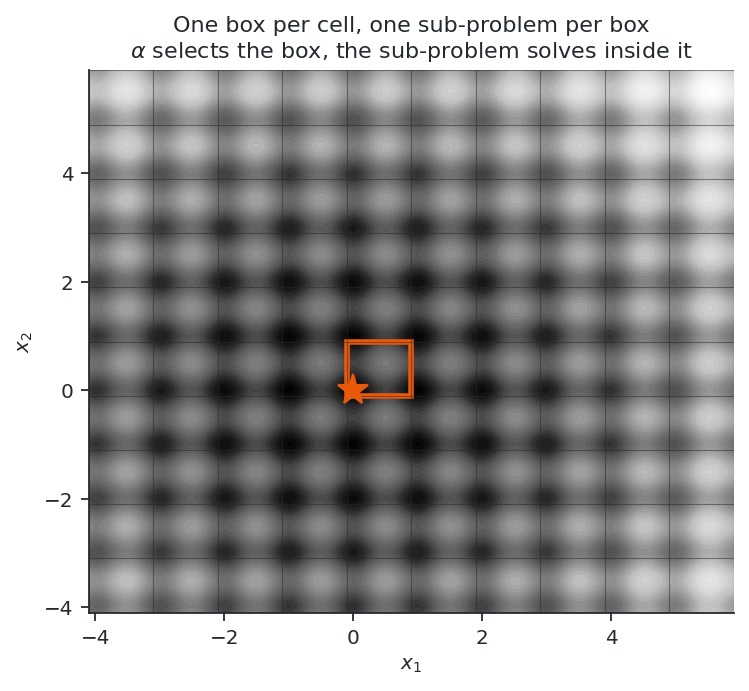
\includegraphics[width=0.48\linewidth]{figures/subdivision.png}\hfill
  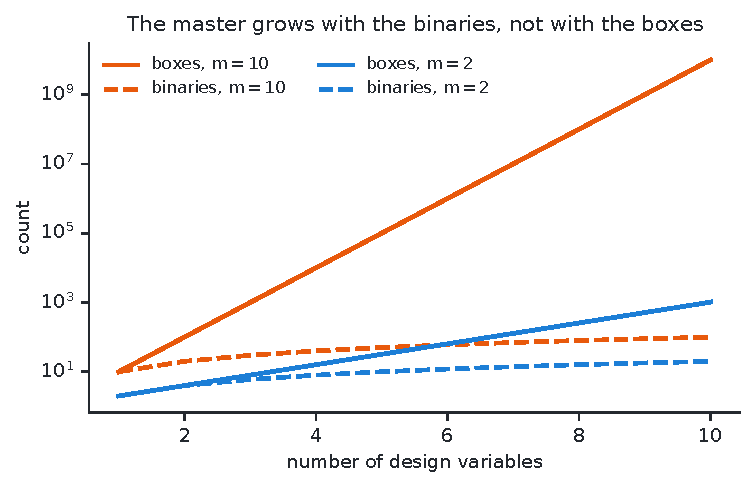
\includegraphics[width=0.48\linewidth]{figures/complexity.pdf}
  \caption{Left: Cartesian subdivision of a two-dimensional design space.
    Right: number of boxes $\prod_j m_j$ and number of binary variables of the
    master problem $\sum_j m_j$ as functions of the number of design
    variables.}
  \label{fig:subdivision}
\end{figure}

\subsection{Encoding of the box selection}

A categorical variable is associated with each component and encoded as a
one-hot vector $\alpha_j \in \{0,1\}^{m_j}$ with $\sum_k \alpha_{j,k} = 1$. The
bounds of the selected box are affine functions of $\alpha$:
\begin{equation}\label{eq:bounds}
  \ell_j(\alpha) = \sum_{k} l_{j,k}\,\alpha_{j,k},
  \qquad
  u_j(\alpha) = \sum_{k} u_{j,k}\,\alpha_{j,k}.
\end{equation}
The master problem thus involves $\sum_j m_j$ binary variables, whereas the
number of boxes is $\prod_j m_j$ (Fig.~\ref{fig:subdivision}, right).

\subsection{Bi-level problem and outer approximation}

Problem~\eqref{eq:problem} is reformulated as
\begin{equation}\label{eq:bilevel}
  \min_{\alpha}\ v(\alpha),
  \qquad
  v(\alpha) = \min_{x} \bigl\{ f(x) : g(x) \le 0,\ \ell(\alpha) \le x \le u(\alpha) \bigr\}.
\end{equation}
The lower-level problem is solved by a local gradient-based optimizer started at
the centre of the box, and the upper-level problem by a mixed-integer master
problem (Fig.~\ref{fig:bilevel}). The value $v(\alpha^{(i)})$ returned by the
local optimizer is an upper bound of the optimum within the box. When a box
contains no point satisfying $g \le 0$, a feasibility cut is returned in addition
to the objective cut, and the box is excluded from the master problem.

After the solution of $N$ sub-problems, the master problem contains the cuts
\begin{equation}\label{eq:cuts}
  \eta \ \ge\ v(\alpha^{(i)}) + s^{(i)\top}\bigl(\alpha - \alpha^{(i)}\bigr),
  \qquad
  s^{(i)} = \left.\frac{\mathrm{d}v}{\mathrm{d}\alpha}\right|_{\alpha^{(i)}},
  \qquad i = 1, \dots, N,
\end{equation}
and $\eta$ is minimized over the one-hot polytope, subject to a trust region
around the incumbent box (Section~\ref{sec:trust}). The lower envelope of the
cuts,
$\hat v(\alpha) = \max_i [v(\alpha^{(i)}) + s^{(i)\top}(\alpha-\alpha^{(i)})]$, is
defined for every box, whether it has been solved or not, and is used by the
master problem to rank the boxes not yet solved. The efficiency of the
exploration therefore depends on the accuracy of the slopes $s^{(i)}$. The
procedure is summarized in Algorithm~\ref{alg:bsoa}.

\begin{figure}[t]
  \centering
  \resizebox{\linewidth}{!}{% Exchanges between the master problem and the sub-problem (Fig. bilevel).
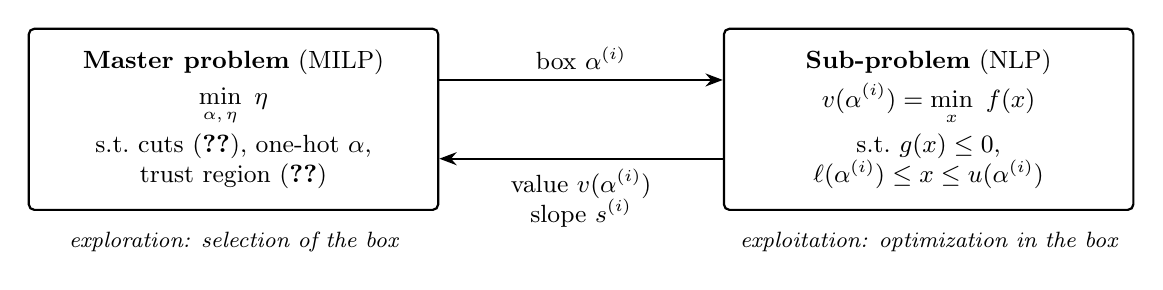
\begin{tikzpicture}[
    font=\small,
    level/.style={draw, thick, rounded corners=2pt, align=center,
                  minimum width=5.2cm, minimum height=2.3cm, inner sep=6pt},
    flow/.style={-{Stealth[length=2.2mm]}, thick},
  ]
  \node[level] (master) {%
    \textbf{Master problem} (MILP)\\[2pt]
    $\displaystyle\min_{\alpha,\,\eta}\ \eta$\\[2pt]
    s.t.\ cuts~\eqref{eq:cuts}, one-hot $\alpha$,\\
    trust region~\eqref{eq:trust}};
  \node[level, right=3.6cm of master] (sub) {%
    \textbf{Sub-problem} (NLP)\\[2pt]
    $\displaystyle v(\alpha^{(i)}) = \min_{x}\ f(x)$\\[2pt]
    s.t.\ $g(x) \le 0$,\\
    $\ell(\alpha^{(i)}) \le x \le u(\alpha^{(i)})$};
  \draw[flow] ([yshift=5mm]master.east) -- node[above, align=center]
    {box $\alpha^{(i)}$} ([yshift=5mm]sub.west);
  \draw[flow] ([yshift=-5mm]sub.west) -- node[below, align=center]
    {value $v(\alpha^{(i)})$\\slope $s^{(i)}$}
    ([yshift=-5mm]master.east);
  \node[below=1.5mm of master, font=\footnotesize\itshape]
    {exploration: selection of the box};
  \node[below=1.5mm of sub, font=\footnotesize\itshape]
    {exploitation: optimization in the box};
\end{tikzpicture}
}
  \caption{Exchanges between the master problem, a mixed-integer linear program
    (MILP) which selects the box $\alpha^{(i)}$, and the sub-problem, a nonlinear
    program (NLP) which returns the local optimum $v(\alpha^{(i)})$ in this box and
    its sensitivity $s^{(i)}$, from which a new cut is built.}
  \label{fig:bilevel}
\end{figure}

\begin{algorithm}[t]
  \caption{Box-subdivision outer approximation}\label{alg:bsoa}
  \begin{algorithmic}[1]
    \Require subdivision $\{[l_{j,k},u_{j,k}]\}$, initial box $\alpha^{(1)}$,
      number of probes $p$, initial trust-region radius $\Delta$
    \State solve the sub-problem in $\alpha^{(1)}$; store $(v^{(1)}, s^{(1)})$;
      incumbent $\bar\alpha \gets \alpha^{(1)}$
    \While{budget not exhausted and stopping criteria not met}
      \State correct the slopes $s^{(i)}$ against non-convexity
        (Section~\ref{sec:convexification})
      \For{each probe $q = 1, \dots, p$ \textbf{in parallel}}
        \State solve the master problem with cuts~\eqref{eq:cuts} and a trust
          region of radius $\Delta_q \in [\Delta/2, \Delta]$ around $\bar\alpha$
        \State solve the sub-problem in the proposed box; store $(v, s)$
      \EndFor
      \State update the incumbent $\bar\alpha$; reduce $\Delta$ if no improvement
    \EndWhile
    \State \Return the best local solution found
  \end{algorithmic}
\end{algorithm}

\subsection{Formulation of the sub-problem}\label{sec:formulations}

The sensitivity of the optimal value with respect to a parameter $p$ is given by
post-optimal analysis as
\begin{equation}\label{eq:postopt}
  \frac{\mathrm{d} f(x^\ast(p), p)}{\mathrm{d}p}
  = \frac{\partial f}{\partial p} + \lambda^\top \frac{\partial g}{\partial p},
\end{equation}
where $\lambda$ denotes the Lagrange multipliers of the constraints. In
Eq.~\eqref{eq:postopt}, the bounds of the design variables are assumed to be
independent of $p$, whereas in problem~\eqref{eq:bilevel} the bounds are
precisely the quantities that depend on $\alpha$. The sub-problem is therefore
formulated so that this assumption is satisfied.

The sub-problem is solved with respect to the normalized variables
$\xi \in [0,1]^n$, with
$x(\xi,\alpha) = \ell(\alpha) + \xi \odot (u(\alpha) - \ell(\alpha))$. The bounds
of the sub-problem are then the unit interval for every box, and the slope is
given by the partial derivative
\begin{equation}\label{eq:slope-normalized}
  \frac{\partial v}{\partial \alpha_{j,k}}
  = \frac{\partial f}{\partial x_j}\,\bigl[(1-\xi_j)\,l_{j,k} + \xi_j\,u_{j,k}\bigr].
\end{equation}
This expression is valid both at an interior optimum, where the gradient
vanishes, and on a face of the box, where $\xi_j$ is fixed at one of its bounds.
In this formulation, the box selection enters the objective function through a
bilinear mapping, and feasibility with respect to the box is satisfied by
construction.

\subsection{Safeguards against non-convexity}\label{sec:convexification}

The cuts~\eqref{eq:cuts} are supporting hyperplanes only if $v$ is convex with
respect to the relaxed variables $\alpha$. This condition is not satisfied for a
multimodal problem. A cut built at one box may then lie above $v$ at another box
and exclude the global optimum, in which case the master problem converges
rapidly to a wrong box without any error being reported. Two safeguards are
therefore considered.

\paragraph{Convexification constant.} In the first approach, a term which is
convex with respect to the relaxed one-hot variables and vanishes at every
integer point is added to the value function:
\begin{equation}\label{eq:convexification}
  \tilde v(\alpha) = v(\alpha) + \kappa\, C(\alpha),
  \qquad
  C(\alpha) = \frac{1}{n_c}\sum_{j}\sum_{k} \alpha_{j,k}(\alpha_{j,k}-1),
\end{equation}
where $n_c$ is the number of categorical components
(Fig.~\ref{fig:convexification}). Since $C = 0$ for every one-hot vector, the
discrete problem is unchanged, while for a sufficiently large value of $\kappa$
the non-convexity of $v$ over the relaxed polytope is compensated. In practice,
only the slopes are modified, according to
$s^{(i)} \gets s^{(i)} + (\kappa/n_c)(2\alpha^{(i)} - 1)$. % TODO: check whether this term is introduced in Barjhoux et al. (2022); if so, cite it here.
This term, which is implemented in the master problem of
\code{gemseo-bilevel-outer-approximation} \citep{gemseobilevel}, has the form of the underestimator of the $\alpha$BB method
\citep{androulakis1995,adjiman1998} applied to the relaxed binary variables,
whose bounds are $0$ and $1$. It is therefore applied in the space of the box
selection and not in that of the design variables $x$. As a consequence, no
bound on the Hessian of $f$ is available to determine $\kappa$, and the term does
not become tighter as the boxes become smaller.

\paragraph{Adaptive repair.} In the second approach, the slopes are corrected on
the basis of the values already computed. For every pair of solved boxes, the
cut built at $\alpha^{(i)}$ is required not to overestimate the value observed at
$\alpha^{(j)}$:
\begin{equation}\label{eq:adaptive}
  v(\alpha^{(i)}) + s^{(i)\top}\bigl(\alpha^{(j)} - \alpha^{(i)}\bigr)
  \le v(\alpha^{(j)}) - \delta,
\end{equation}
where $\delta$ is a convexity margin. The violations of these conditions are
removed by a correction of the slopes, which is computed independently for each
cut. For the cut built at $\alpha^{(i)}$, the matrix of the displacements towards
the $N$ solved boxes and the vector of the excesses of the cut over the
condition~\eqref{eq:adaptive} are defined as
\begin{align}
  D_i &= \bigl[\alpha^{(1)} - \alpha^{(i)}, \dots, \alpha^{(N)} - \alpha^{(i)}\bigr],
  \label{eq:repair-data}\\
  r_{i,j} &= \max\Bigl(0,\ s^{(i)\top}\bigl(\alpha^{(j)} - \alpha^{(i)}\bigr)
    - \bigl[v(\alpha^{(j)}) - v(\alpha^{(i)})\bigr] + \delta\Bigr),
  \qquad j = 1, \dots, N,
  \label{eq:repair-excess}
\end{align}
so that $r_{i,j} > 0$ if and only if the cut built at $\alpha^{(i)}$ violates
condition~\eqref{eq:adaptive} at $\alpha^{(j)}$. The corrected slope is
\begin{equation}\label{eq:repair}
  \tilde s^{(i)} = s^{(i)} - D_i\,\mu_i,
  \qquad
  \mu_i \in \operatorname*{arg\,min}_{\mu \in \R^{N}}
    \bigl\| D_i^\top D_i\,\mu - r_i \bigr\|_2 ,
\end{equation}
where the minimum-norm solution of the least-squares problem is retained. When
the system $D_i^\top D_i\,\mu = r_i$ is consistent,
$\tilde s^{(i)\top}(\alpha^{(j)} - \alpha^{(i)})
 = s^{(i)\top}(\alpha^{(j)} - \alpha^{(i)}) - r_{i,j}$
for every $j$, so that the violated conditions~\eqref{eq:adaptive} are satisfied
with equality, the other ones are left unchanged, and the correction
$D_i\,\mu_i$ is the correction of minimum Euclidean norm with this property. The
boxes whose sub-problem is infeasible are included among the $N$ solved boxes,
and the same correction is applied to the cuts of the inequality constraints.
The corrected slopes $\tilde s^{(i)}$ are then used in place of $s^{(i)}$ in the
cuts~\eqref{eq:cuts} (Fig.~\ref{fig:repair}).

The two approaches can be combined in principle; they are used separately in
this work. With a large value of $\kappa$, the cuts are valid by construction,
but the lower bound of the master problem is decreased by approximately
$\kappa$, so that the optimality gap cannot close. Moreover, when $\kappa$
exceeds the value required to compensate the non-convexity, every box not yet
solved is ranked before the incumbent, and the method tends towards an
enumeration of the boxes. The constant therefore has a useful range bounded on
both sides.

With the adaptive repair, the lower bound is not degraded by a uniform shift.
Convexity is, however, enforced only with respect to the boxes already solved,
and no convergence guarantee is obtained. For values of $\delta$ below a
threshold, the cuts remain invalid. Conversely, when $\delta$ exceeds the range
of the objective function, the right-hand side of the least-squares problem is
dominated by the margin rather than by the observed values, all slopes are
shifted in the same direction, and the ranking of the boxes no longer reflects
the landscape.

\begin{figure}[t]
  \centering
  % Convexification term over a relaxed one-hot variable (Fig. convexification).
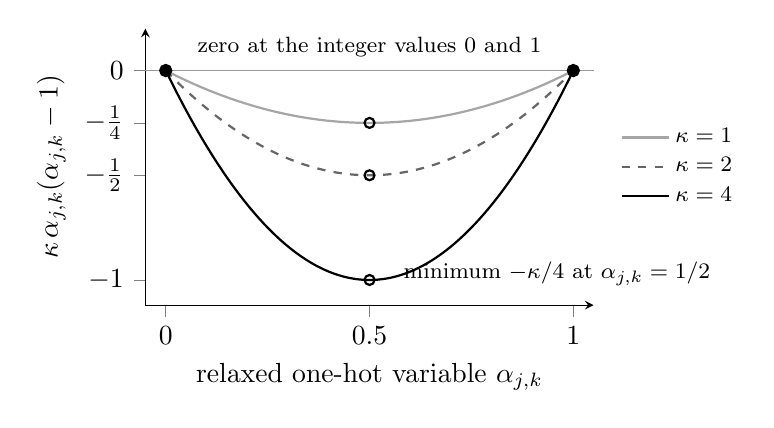
\begin{tikzpicture}
  \begin{axis}[
      width=0.6\linewidth, height=0.42\linewidth,
      xmin=-0.05, xmax=1.05, ymin=-1.12, ymax=0.2,
      xtick={0,0.5,1}, ytick={-1,-0.5,-0.25,0},
      yticklabels={$-1$,$-\tfrac12$,$-\tfrac14$,$0$},
      xlabel={relaxed one-hot variable $\alpha_{j,k}$},
      ylabel={$\kappa\,\alpha_{j,k}(\alpha_{j,k}-1)$},
      axis lines=left, tick align=outside, clip=false,
      legend style={draw=none, fill=none, font=\footnotesize,
                    at={(1.04,0.5)}, anchor=west},
      legend cell align=left,
      every axis plot/.append style={thick, domain=0:1, samples=101},
    ]
    \draw[black!40, thin] (axis cs:-0.05,0) -- (axis cs:1.05,0);
    \addplot[black!35] {1*x*(x-1)};  \addlegendentry{$\kappa = 1$}
    \addplot[black!60, dashed] {2*x*(x-1)};  \addlegendentry{$\kappa = 2$}
    \addplot[black] {4*x*(x-1)};  \addlegendentry{$\kappa = 4$}
    \addplot[only marks, mark=*, mark size=2pt, black, forget plot]
      coordinates {(0,0) (1,0)};
    \addplot[only marks, mark=o, mark size=1.8pt, black, forget plot]
      coordinates {(0.5,-0.25) (0.5,-0.5) (0.5,-1)};
    \node[font=\footnotesize, anchor=south] at (axis cs:0.5,0.02)
      {zero at the integer values $0$ and $1$};
    \node[font=\footnotesize, anchor=west] at (axis cs:0.56,-0.97)
      {minimum $-\kappa/4$ at $\alpha_{j,k} = 1/2$};
  \end{axis}
\end{tikzpicture}

  \caption{Contribution $\kappa\,\alpha_{j,k}(\alpha_{j,k}-1)$ of one relaxed
    one-hot variable to the convexification term $\kappa C(\alpha)$, for three
    values of $\kappa$. The term vanishes at the integer values, so that the
    discrete problem is unchanged, and lowers the relaxation between them by up
    to $\kappa/4$.}
  \label{fig:convexification}
\end{figure}

\begin{figure}[t]
  \centering
  % Adaptive repair of one cut (Fig. adaptive-repair). The cut built at the box
% i = 2 is evaluated at the other solved boxes; where it exceeds v - delta, the
% repaired slope lowers it to v - delta, and the other values are unchanged.
% Values: v = (5.0, 3.2, 4.1, 1.8, 3.2, 2.0, 4.4), delta = 0.4, cut values
% (1.7, 3.2, 5.1, 3.7, 2.6, 1.6, 3.5); the boxes 3 and 4 are violated.
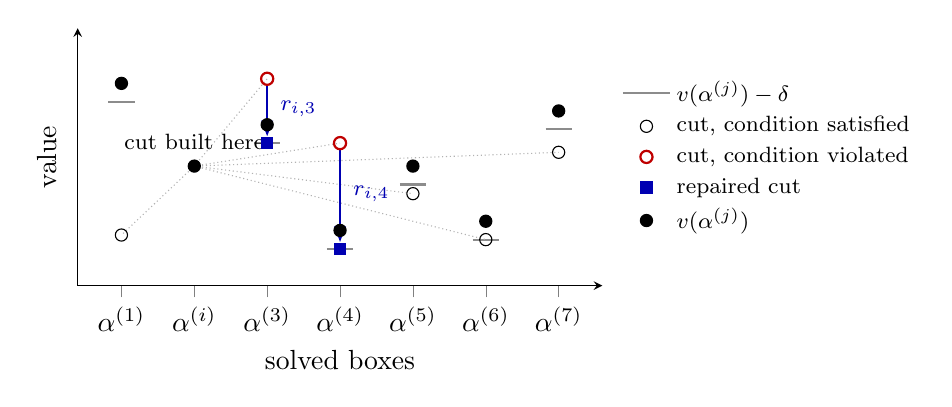
\begin{tikzpicture}
  \begin{axis}[
      width=0.68\linewidth, height=0.4\linewidth,
      xmin=0.4, xmax=7.6, ymin=0.6, ymax=6.2,
      xtick={1,...,7},
      xticklabels={$\alpha^{(1)}$,$\alpha^{(i)}$,$\alpha^{(3)}$,$\alpha^{(4)}$,
                   $\alpha^{(5)}$,$\alpha^{(6)}$,$\alpha^{(7)}$},
      ytick=\empty,
      xlabel={solved boxes}, ylabel={value},
      axis lines=left, tick align=outside, clip=false,
      legend style={draw=none, fill=none, font=\footnotesize,
                    at={(1.02,0.5)}, anchor=west},
      legend cell align=left,
    ]
    % Margin delta below every observed value.
    \foreach \j/\v in {1/5.0, 3/4.1, 4/1.8, 5/3.2, 6/2.0, 7/4.4}{
      \edef\temp{\noexpand\draw[black!45, thick]
        (axis cs:\j-0.18,\v-0.4) -- (axis cs:\j+0.18,\v-0.4);}
      \temp}
    \addlegendimage{black!45, thick}
    \addlegendentry{$v(\alpha^{(j)}) - \delta$}
    % Cut before the repair, joined to its own box for readability.
    \foreach \j/\c in {1/1.7, 3/5.1, 4/3.7, 5/2.6, 6/1.6, 7/3.5}{
      \edef\temp{\noexpand\draw[black!30, densely dotted]
        (axis cs:2,3.2) -- (axis cs:\j,\c);}
      \temp}
    \addplot[only marks, mark=o, mark size=2.2pt, black]
      coordinates {(1,1.7) (5,2.6) (6,1.6) (7,3.5)};
    \addlegendentry{cut, condition satisfied}
    \addplot[only marks, mark=o, mark size=2.2pt, red!75!black, thick]
      coordinates {(3,5.1) (4,3.7)};
    \addlegendentry{cut, condition violated}
    \addplot[only marks, mark=square*, mark size=2pt, blue!70!black]
      coordinates {(3,3.7) (4,1.4)};
    \addlegendentry{repaired cut}
    \addplot[only marks, mark=*, mark size=2.2pt, black]
      coordinates {(1,5.0) (2,3.2) (3,4.1) (4,1.8) (5,3.2) (6,2.0) (7,4.4)};
    \addlegendentry{$v(\alpha^{(j)})$}
    % Corrections r_ij of the violated conditions.
    \draw[-{Stealth[length=2mm]}, blue!70!black, thick]
      (axis cs:3,4.95) -- (axis cs:3,3.85);
    \draw[-{Stealth[length=2mm]}, blue!70!black, thick]
      (axis cs:4,3.55) -- (axis cs:4,1.55);
    \node[font=\footnotesize, anchor=west, blue!70!black] at (axis cs:3.05,4.45)
      {$r_{i,3}$};
    \node[font=\footnotesize, anchor=west, blue!70!black] at (axis cs:4.05,2.6)
      {$r_{i,4}$};
    \node[font=\footnotesize, anchor=south] at (axis cs:2,3.35)
      {cut built here};
  \end{axis}
\end{tikzpicture}

  \caption{Adaptive repair of the cut built at the box $\alpha^{(i)}$,
    schematic. The cut is evaluated at the other solved boxes. Where it exceeds
    $v(\alpha^{(j)}) - \delta$, condition~\eqref{eq:adaptive} is violated, and
    the corrected slope lowers it by the excess $r_{i,j}$ to
    $v(\alpha^{(j)}) - \delta$; its values at the other boxes are unchanged. The
    dotted segments only join the cut to its own box: since the boxes are
    vertices of the relaxed polytope, the cut is not a line through them.}
  \label{fig:repair}
\end{figure}

\paragraph{Swept convexity.} Both $\kappa$ and $\delta$ are expressed in the
units of the objective function, and have to be specified before any information
on this function is available, whereas a suitable value depends on the range of
the function. To avoid this calibration, the parallel probes of the master problem,
which are already used to sweep the trust-region radius, are also used to sweep
the convexity value, which is by default the margin $\delta$ of the adaptive
repair. A sequence of values $\delta_1 < \dots < \delta_p$, referred
to as a ladder and distributed geometrically below an upper bound, is defined,
and one value is assigned to each probe (Fig.~\ref{fig:sweep}). The values are paired with the radii so
that the smallest radii are associated with the least corrected cuts and the
largest radii with the most corrected ones, and each iteration therefore
proposes both boxes close to the incumbent and distant boxes. When a probe
proposes a box which has already been solved, the next value of the ladder is
assigned to it, at the cost of one additional mixed-integer solution and without
any evaluation of the objective function. The run is terminated when the ladder
is exhausted for all probes.

The upper bound of the ladder is set to ten times the spread of the objective
values over the boxes already solved, including the infeasible ones. The factor
compensates for the underestimation of the spread when the first boxes are few
and similar. It is dimensionless and can therefore be applied to other problems,
contrary to an absolute margin. It should be noted that the sweep does
not restore the optimality test, since the master problem retains the smallest
lower bound among the probes, which is degraded by the largest convexity values.

\begin{figure}[t]
  \centering
  % Swept margin delta of the adaptive repair with four probes (Fig. sweep). The rungs are geometric, so
% that they are equally spaced on the logarithmic axis; the probe k starts at
% the rung k with the k-th radius, and the probe 2 climbs one rung because the
% box it proposed has already been solved.
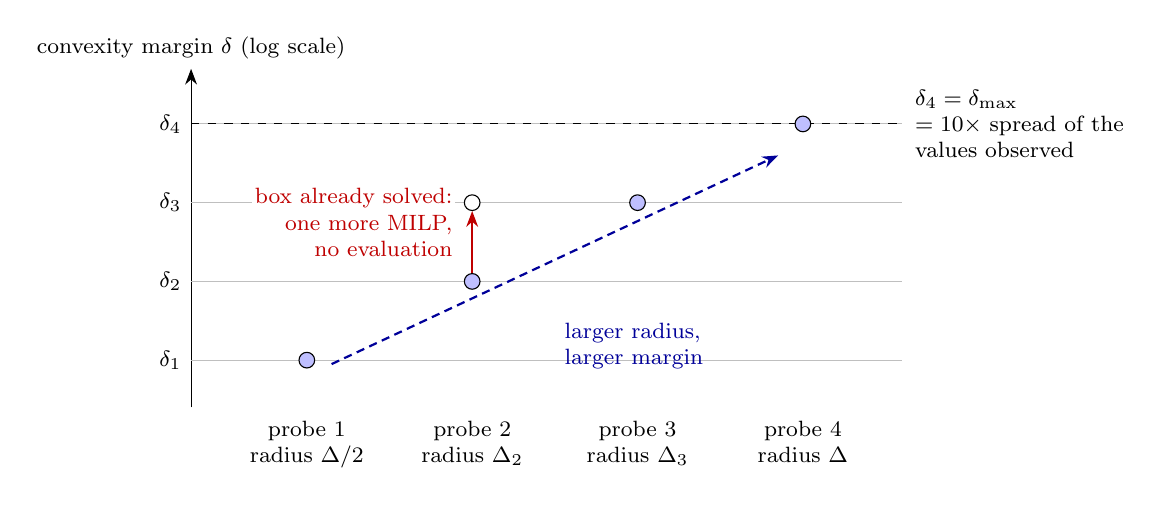
\begin{tikzpicture}[x=2.1cm, y=1.0cm, font=\footnotesize]
  % Logarithmic axis of the convexity value.
  \draw[-{Stealth[length=2mm]}] (0.3,0.4) -- (0.3,4.7)
    node[above] {convexity margin $\delta$ ($\log$ scale)};
  \foreach \k in {1,...,4}{
    \draw[black!25] (0.3,\k) -- (4.6,\k);
    \node[left] at (0.3,\k) {$\delta_{\k}$};}
  \draw[black, dashed] (0.3,4) -- (4.6,4);
  \node[anchor=west, align=left] at (4.62,4)
    {$\delta_4 = \delta_{\max}$\\$= 10\times$ spread of the\\values observed};
  % Probes, each at its own rung and radius.
  \foreach \k/\radius in {1/{\Delta/2}, 2/{\Delta_2}, 3/{\Delta_3}, 4/{\Delta}}{
    \node[draw, circle, fill=blue!25, inner sep=2pt] (p\k) at (\k,\k) {};
    \node[below, align=center] at (\k,0.35)
      {probe \k\\radius $\radius$};}
  % Probe 2 proposes a solved box and climbs to the next rung.
  \node[draw, circle, fill=white, inner sep=2pt] (q2) at (2,3) {};
  \draw[-{Stealth[length=2mm]}, red!75!black, thick] (p2) -- (q2);
  \node[anchor=east, align=right, red!75!black, fill=white, inner sep=1pt] at (1.9,2.75)
    {box already solved:\\one more MILP,\\no evaluation};
  % Pairing of the radii and the rungs.
  \draw[blue!60!black, thick, densely dashed, -{Stealth[length=2mm]}]
    (1.15,0.95) -- (3.85,3.6);
  \node[anchor=north west, align=left, blue!60!black] at (2.5,1.6)
    {larger radius,\\larger margin};
\end{tikzpicture}

  \caption{Swept convexity margin $\delta$ of the adaptive repair with four
    probes, schematic. The values of the
    ladder are geometric below $\delta_{\max}$, ten times the spread of the
    objective values over the boxes already solved, and each probe starts at its
    own value, the radius of its trust region increasing with the value. A probe
    which proposes a box already solved is given the next value of the ladder,
    at the cost of one mixed-integer solution and without evaluation of the
    objective function.}
  \label{fig:sweep}
\end{figure}

\subsection{Trust region of the master problem}\label{sec:trust}

The search of the master problem is restricted to a neighbourhood of the
incumbent box $\bar\alpha$:
\begin{equation}\label{eq:trust}
  \operatorname{card}\{\, j : \alpha_j \ne \bar\alpha_j \,\} \ \le\ \Delta,
\end{equation}
where $\alpha_j$ denotes the interval selected for the component $j$, and the
left-hand side is linear in the one-hot variables. The radius $\Delta$ bounds the Hamming distance between the selected intervals,
i.e. the number of modified components, and constraint~\eqref{eq:trust} becomes a local branching constraint
\citep{fischetti2003}. A radius of one admits the boxes which differ from the
incumbent in a single component, and a radius of $\Delta$ admits
$\sum_{k=0}^{\Delta}\binom{n}{k}(m-1)^k$ boxes for $n$ components subdivided into
$m$ intervals each (Fig.~\ref{fig:trust}). The Hamming distance treats the box
selection as a categorical choice; an ordinal variant,
$|v^\top\alpha - v^\top\bar\alpha| \le \Delta$, where $v$ denotes the interval
indices, is compared with it in Section~\ref{sec:mechanisms}.

The initial radius is set to $\Delta = 2$ (Section~\ref{sec:mechanisms}). The
radius is multiplied by $0.7$ after a given number
of iterations without improvement, down to a minimum value of one. Once this
value is reached, the radii of the probes, which lie in $[\Delta/2, \Delta]$,
coincide, all probes solve the same master problem, and the exploration stops.

\paragraph{Euclidean trust region.} As an alternative, the Euclidean distance
between the centre $c(\alpha)$ of a candidate box and that of the incumbent box
can be bounded. In the design space scaled to the unit hypercube, the squared
distance
\begin{equation}\label{eq:euclidean}
  \|c(\alpha) - c(\bar\alpha)\|^2
  = \sum_j \sum_k \alpha_{j,k}\,\bigl(c_{j,k} - c_j(\bar\alpha)\bigr)^2,
\end{equation}
where $c_{j,k}$ denotes the centre of the interval $k$ of the component $j$, is
linear in the one-hot variables, since one of them is equal to one for each
component, so that the trust region remains a linear constraint of the master
problem. Two schedules of the radius $R$ are considered. In the first one, $R$
starts at a fixed value and follows the reduction rule of the Hamming radius. In
the second one, $R$ starts at the diameter of the subdivision, so that the region
initially covers every box, and the radii of the probes are distributed from
$R/(2\sqrt{n})$ to $R$, with a lower bound of one interval width, which keeps the
probes distinct. In a third variant, a candidate is admitted when it lies within
the radius of any evaluated box rather than of the incumbent: the region is then
a union of balls, which is expressed with one additional binary variable per
evaluated box.

\begin{figure}[t]
  \centering
  % Hamming trust regions of radius 1 and 2 around the incumbent (7,6),
% ten subdivisions per variable.
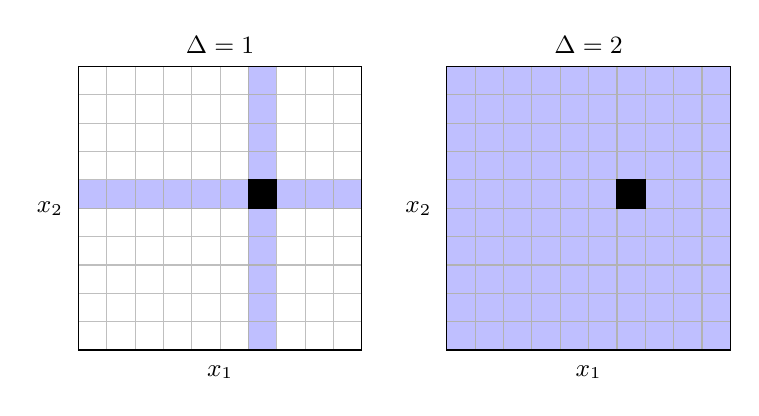
\begin{tikzpicture}[x=0.36cm,y=0.36cm,font=\small]
  \foreach \panel/\radius/\shift in {a/1/0, b/2/13}{
    \begin{scope}[xshift=\shift cm*0.36]
      \foreach \i in {1,...,10}{
        \foreach \j in {1,...,10}{
          \pgfmathtruncatemacro{\changed}{(\i!=7)+(\j!=6)}
          \ifnum\changed>\radius\relax
            \draw[gray!50,fill=white] (\i-1,\j-1) rectangle ++(1,1);
          \else
            \draw[gray!60,fill=blue!25] (\i-1,\j-1) rectangle ++(1,1);
          \fi
        }
      }
      \draw[fill=black] (6,5) rectangle ++(1,1);
      \draw (0,0) rectangle (10,10);
      \node[below] at (5,-0.2) {$x_1$};
      \node[left] at (-0.2,5) {$x_2$};
      \node[above] at (5,10.1) {$\Delta = \radius$};
    \end{scope}
  }
\end{tikzpicture}

  \caption{Trust regions around the incumbent box (black), with ten
    subdivisions per variable; the admitted boxes are shaded. Top: Hamming
    distance, the admitted boxes differing from the incumbent in at most
    $\Delta$ components; in two dimensions, a radius of two admits the whole
    design space. Bottom: Euclidean distance between box centres, in interval
    widths. Left to right: a ball of radius two; the diameter schedule at its
    initial radius, whose smallest probe admits the boxes within the circle and
    whose largest probe admits the whole design space (light shading); and the
    union of the balls of radius $1.5$ around the evaluated boxes (grey and
    black).}
  \label{fig:trust}
\end{figure}

\subsection{Density of the subdivision}\label{sec:density}

The admissible values of the subdivision density $m_j$ are bounded from above
and from below.

\paragraph{Upper bound.} With a budget of a few thousand evaluations, a few dozen
sub-problems can be solved, which provides a few dozen cuts to identify a cut
model with $\sum_j m_j$ coefficients. The admissible density is therefore
limited by the ratio between the number of binary variables and the number of
affordable cuts, and not by the number of boxes.

\paragraph{Lower bound.} The subdivision must separate the basins of attraction.
For instance, minima one unit apart over a range of ten require about ten
intervals. When the lower bound exceeds the upper bound, the method cannot be
applied.

\paragraph{Estimation of the density.} Since the density has to follow the
spacing of the basins, the expected number of minima along an axial line,
\begin{equation}\label{eq:basins}
  N_j = \mathbb{E}_{x_\perp}\Bigl[\#\bigl\{t : \partial_j f(x_\perp + t e_j) = 0,\ \partial_{jj} f > 0\bigr\}\Bigr],
\end{equation}
is estimated, and the density is set to $m_j = N_j$. Contrary to a wavelength,
this quantity is defined for any continuously differentiable function. The
expectation is estimated by Monte Carlo sampling over random anchor points
$x_\perp$, and the abscissae along each line are also drawn at random, since a
uniform sampling may resonate with a regular landscape and return a consistent
but wrong count. A minimum is retained when its topographic prominence, measured
with respect to the saddle that closes its basin, exceeds a given fraction of the
range of the scan. A space-filling design cannot be used instead of the axial
scans, since averaging over the other components yields the main effect
$\mathbb{E}[f \mid x_j]$, in which the multimodality due to interactions between
variables, as for the Griewank and Ackley functions, disappears. A scan can only
reveal the basins that it resolves, so that the estimate is a lower bound of
$N_j$, and no upper bound can be obtained from a finite sample. When the counts
obtained with increasing sampling rates do not converge, the estimate is
therefore reported as unresolved. For constrained problems, the same count is
applied to the restriction of $f$ to each maximal feasible interval of the line.

\subsection{Extensions}\label{sec:extensions}

Three extensions related to the limits on the density were also studied
(Fig.~\ref{fig:subdivision-variants}). They are evaluated in
Section~\ref{sec:extensions-results} and are not used by default.

\begin{figure}[t]
  \centering
  % Variants of the subdivision in two dimensions (Fig. subdivision-variants):
% partial subdivision, multi-resolution encoding with two levels of four
% intervals, hierarchy with two levels of four intervals, and deep hierarchy of
% three levels of two intervals. The selected box is dark, the boxes reachable
% by one master problem are drawn, and the coarse box containing the selected
% box is light.
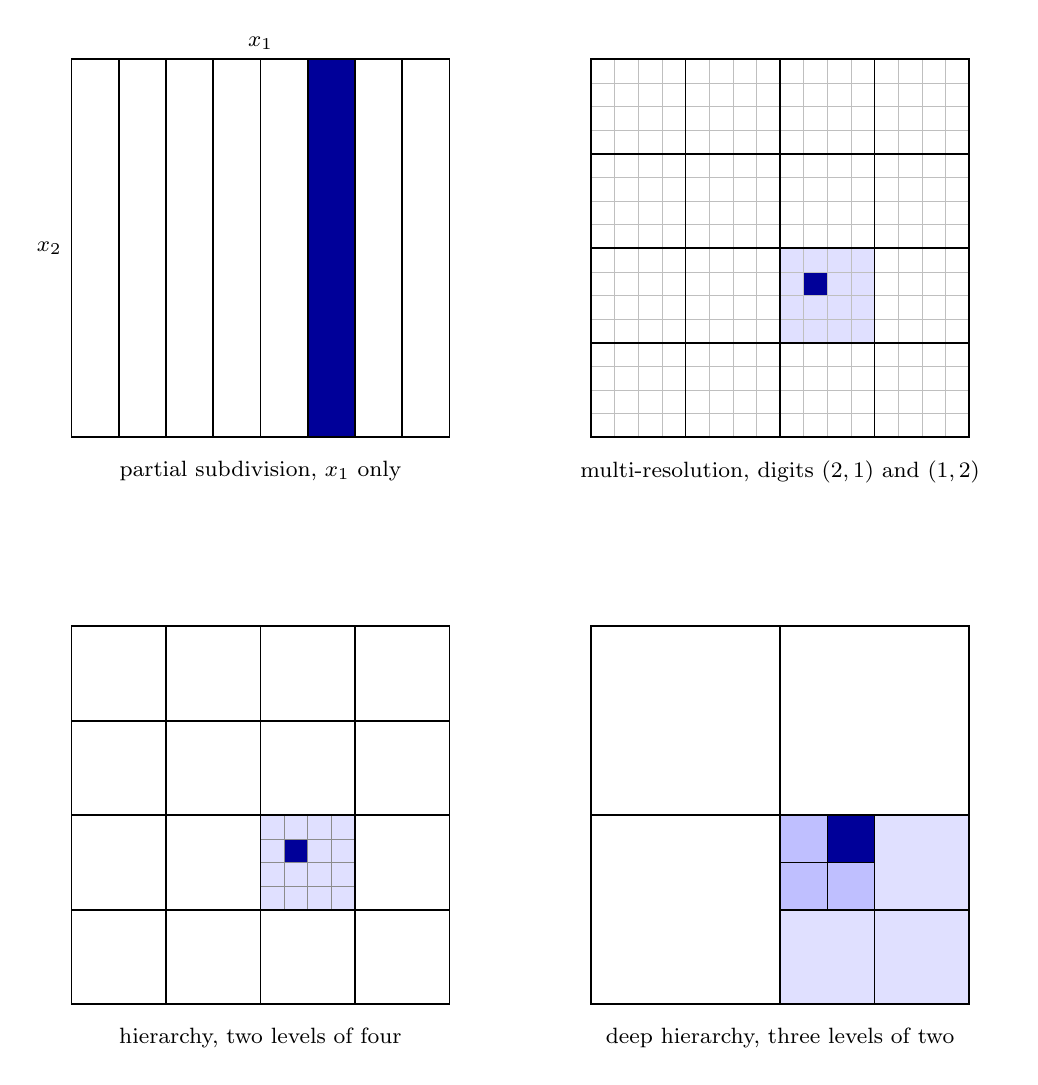
\begin{tikzpicture}[x=0.3cm, y=0.3cm, font=\footnotesize]
  \tikzset{
    fine/.style={black!25, very thin},
    coarse/.style={black, semithick},
    chosen/.style={fill=blue!60!black},
    parent/.style={fill=blue!12},
  }
  \newcommand{\panel}[1]{%
    \draw[coarse] (0,0) rectangle (16,16);
    \node[below, align=center, text width=5.6cm] at (8,-0.6) {#1};}
  % --- Partial subdivision: x1 in eight intervals, x2 continuous.
  \begin{scope}
    \fill[chosen] (10,0) rectangle (12,16);
    \foreach \i in {2,4,...,14}{\draw[coarse] (\i,0) -- (\i,16);}
    \panel{partial subdivision, $x_1$ only}
    \node[left] at (0,8) {$x_2$};
    \node[above] at (8,16) {$x_1$};
  \end{scope}
  % --- Multi-resolution: two levels of four intervals, 16 x 16 boxes in one
  % master problem, the box given by one digit per level and per component.
  \begin{scope}[xshift=6.6cm]
    \fill[parent] (8,4) rectangle (12,8);
    \fill[chosen] (9,6) rectangle (10,7);
    \foreach \i in {1,...,15}{
      \draw[fine] (\i,0) -- (\i,16);
      \draw[fine] (0,\i) -- (16,\i);}
    \foreach \i in {4,8,12}{
      \draw[coarse] (\i,0) -- (\i,16);
      \draw[coarse] (0,\i) -- (16,\i);}
    \panel{multi-resolution, digits $(2,1)$ and $(1,2)$}
  \end{scope}
  % --- Hierarchy: a coarse subdivision of four intervals, then the promising
  % box subdivided again into four.
  \begin{scope}[yshift=-7.2cm]
    \fill[parent] (8,4) rectangle (12,8);
    \fill[chosen] (9,6) rectangle (10,7);
    \foreach \i in {9,10,11}{
      \draw[fine, black!45] (\i,4) -- (\i,8);
      \draw[fine, black!45] (8,\i-4) -- (12,\i-4);}
    \foreach \i in {4,8,12}{
      \draw[coarse] (\i,0) -- (\i,16);
      \draw[coarse] (0,\i) -- (16,\i);}
    \panel{hierarchy, two levels of four}
  \end{scope}
  % --- Deep hierarchy: every variable halved at each of three levels.
  \begin{scope}[xshift=6.6cm, yshift=-7.2cm]
    \fill[parent] (8,0) rectangle (16,8);
    \fill[blue!25] (8,4) rectangle (12,8);
    \fill[chosen] (10,6) rectangle (12,8);
    \draw[coarse] (8,0) -- (8,16);
    \draw[coarse] (0,8) -- (16,8);
    \draw[coarse] (12,0) -- (12,8);
    \draw[coarse] (8,4) -- (16,4);
    \draw[coarse] (10,4) -- (10,8);
    \draw[coarse] (8,6) -- (12,6);
    \panel{deep hierarchy, three levels of two}
  \end{scope}
\end{tikzpicture}

  \caption{Extensions of the subdivision in two dimensions, the selected box
    being dark. Top left: subdivision of $x_1$ only, $x_2$ remaining a
    continuous variable of the sub-problem; multi-resolution encoding with two
    levels of four intervals, the $16 \times 16$ boxes being available to one
    master problem, which selects the box by one digit per level and per
    component, numbered from zero (top right); hierarchy with two levels of four
    intervals, the box selected at the first level (light) being subdivided and
    solved in turn (bottom left); and deep hierarchy, every variable being
    halved at each of three levels (bottom right).}
  \label{fig:subdivision-variants}
\end{figure}

\paragraph{Partial subdivision.} Only the variables in which the objective
function is multimodal are subdivided, the other variables being treated as
continuous variables of the sub-problems.

\paragraph{Multi-resolution encoding.} The box is selected by one categorical
variable per level of resolution, the levels providing the base-$m$ digits
$d_k(\alpha_j) \in \{0,\dots,m-1\}$ of the interval index:
\begin{equation}\label{eq:multires}
  \ell_j(\alpha) = L_j + \Delta_j \sum_{k=1}^{L} m^{-k}\, d_k(\alpha_j),
  \qquad
  u_j(\alpha) = \ell_j(\alpha) + \Delta_j\, m^{-L},
  \qquad \Delta_j = U_j - L_j .
\end{equation}
With $L$ levels of $m$ intervals, a resolution of $m^L$ intervals per component
is obtained with $Lm$ binary variables. For instance, two levels of four
intervals provide sixteen intervals per component with eight binary variables
instead of sixteen. Since the width of a box does not depend on the digits, the
Jacobian of the mapping is constant and the post-optimal sensitivity remains
valid. The cut model is linear with respect to the digits and is therefore
additive over the levels, so that the dependence of the effect of a fine digit
on the value of a coarse digit cannot be represented. The trust-region radius is
multiplied by $L$, since a change of interval may modify up to $L$ digits.

\paragraph{Hierarchies of subdivisions.} A coarse subdivision is solved first,
and a promising box is then subdivided and solved in turn. With two levels of
$m^{(1)}$ and $m^{(2)}$ intervals, a resolution of $m^{(1)}m^{(2)}$ is obtained,
while no master problem has more than $\sum_j m_j^{(k)}$ binary variables. Three
variants are considered: a hierarchy with two levels; a deep hierarchy in which
every variable is divided into two intervals at each of $d$ levels, with $2n$
binary variables per level; and a best-first search which keeps the open boxes of
all levels in a priority queue, similar to a spatial branch and bound method in
which the relaxation is replaced by the cut model. Since the cuts of a parent box
are expressed in the one-hot variables of its own subdivision, they are
discarded at each refinement, and a new cut model has to be identified for each
node.

%% ---------------------------------------------------------------------------
\section{Implementation}\label{sec:implementation}

The method is implemented in the open-source package
\code{gemseo-box-subdivision} \citep{boxsubdivision}, a plugin of the GEMSEO
library \citep{gallard2018} based on the \code{Benders} formulation of
\code{gemseo-bilevel-outer-approximation} \citep{gemseobilevel}, which implements
the bi-level outer approximation of \citet{barjhoux2022}. Both levels are
defined in a single catalogue design space, which is split by the formulation,
the categorical variables describing the box selection being assigned to the
master problem. A mapping discipline computes $x(\xi,\alpha)$ with an analytic Jacobian, and is
chained
before the disciplines that compute the objective function. The assembly is
performed by a scenario class, which builds the design space from the
subdivision, chains the mapping, defines the variables of the master problem,
selects the formulation and converts the settings of the method, such as a
trust-region radius expressed in number of modified components, into the
settings of the master problem. The user therefore only provides the
disciplines, the design space and the number of subdivisions. The sub-problems
are solved by SLSQP \citep{kraft1988} for the analytic problems and by MMA
\citep{svanberg1987,gemseomma} for the topology optimization problem, and the master
problem is a mixed-integer linear program.

Each sub-problem is started at the centre of its box, i.e. at $\xi = 1/2$, so
that the result does not depend on the order in which the boxes are solved. The
two safeguards against non-convexity of Section~\ref{sec:convexification} are
used separately: when one of them is selected, the parameter of the other one is
set to zero by default. For versions of the master problem which do not
implement the swept convexity, the sweep is performed by the package outside the
master problem.

The parallel evaluation of the probes reduces the computation time
only when the solution of a sub-problem is expensive compared with that of the
master problem, as for the topology optimization problem.

%% ---------------------------------------------------------------------------
\section{Numerical experiments}\label{sec:results}

\subsection{Test problems and protocol}\label{sec:protocol}

The method is assessed on the Rastrigin \citep{rastrigin1974,torn1989}, Ackley
\citep{ackley1987}, Styblinski--Tang \citep{styblinski1990} and Griewank
\citep{griewank1981} functions \citep[see also][]{jamil2013} in $n = 2$ and
$n = 5$ dimensions, and on a partly multimodal function, defined as the Rastrigin
function in the first two variables and a paraboloid in the other ones
(Appendix~\ref{app:problems}, Fig.~\ref{fig:problems}). The bounds are shifted so
that the global minimizer lies neither at the centre nor on the boundary of a box,
which would favour a method based on a subdivision of the design space. The four
classical functions represent different types of landscape: two well separated
basins per variable for the Styblinski--Tang function, regularly spaced basins
about one unit apart over a range of ten for the Rastrigin function, a single
broad basin with a superimposed oscillation for the Ackley function, and closely
spaced minima of similar values on a shallow paraboloid for the Griewank
function.

The global minimum of each of these functions is known analytically, and the
distance to the optimum reported in the tables is the difference between the best
objective value found and this minimum. All runs are given a fixed budget of
equivalent evaluations, the computation of a
gradient being counted as one evaluation. When the cost of a run is equal to the
budget, the run was stopped by the budget and not by its own stopping criterion.
The distance to the optimum is then an upper bound of the distance that would be
obtained with a larger budget, and such results are marked in the tables. The
variants of the method and the baselines are compared by means of data profiles
\citep{more2009}. For each problem, twenty target values are defined, from a value
reached early by all methods down to the global optimum, and the data profile
gives the fraction of the targets reached, over all problems and starting points,
as a function of the number of evaluations. The targets are generated from the
histories of all runs of a given dimension with \code{gemseo-benchmark}
\citep{gemseobenchmark}, and the configurations are ranked by the area under
their profile.

The following baselines are considered: the multistart algorithm of GEMSEO with
$50$ starting points and SLSQP as local optimizer, which is also the optimizer of
the sub-problems, so that the comparison concerns only the choice of the starting
regions; CMA-ES \citep{hansen2001,hansen2016}, with an initial standard deviation
equal to a quarter of the range; DIRECT \citep{jones1993}, as implemented in SciPy
\citep{virtanen2020}; and efficient global optimization (EGO) \citep{jones1998},
as implemented in \code{egobox} \citep{lafage2022}; and the classic tunneling
method \citep{levy1985}, which alternates SLSQP minimizations with the
minimization of the tunneling function from a random perturbation of the last
minimizer, with a pole at every minimizer found, and spends the whole budget
since it has no other stopping rule. Its settings are fixed choices, not tuned
on these problems, and it was added after the other baselines, from the same
starting points.

\paragraph{Limitations of the protocol.} The configuration of the method compared
with the baselines is the same in both dimensions, but its number of
subdivisions, its trust-region radius and the headroom factor of the sweep were
selected on these problems, from a first study of the variants with five
starting points which are among the twenty of the final comparison, which
introduces a bias in favour of the method. The comparisons of the variants and
with the baselines use twenty starting points per problem and paired
statistical tests with a correction for multiple comparisons
(Sections~\ref{sec:variants} and~\ref{sec:baselines}). The other comparisons use
the same twenty starting points, and a difference of success between two of
their configurations is called significant when the exact McNemar test gives a
$p$-value below $0.05$, without correction for multiple comparisons. The cost of
the master problem is not included in the budget. The results presented below therefore
characterize the method on the problems studied, and an assessment of its general
performance would require an independent set of test problems and a protocol
defined in advance.

\begin{figure}[t]
  \centering
  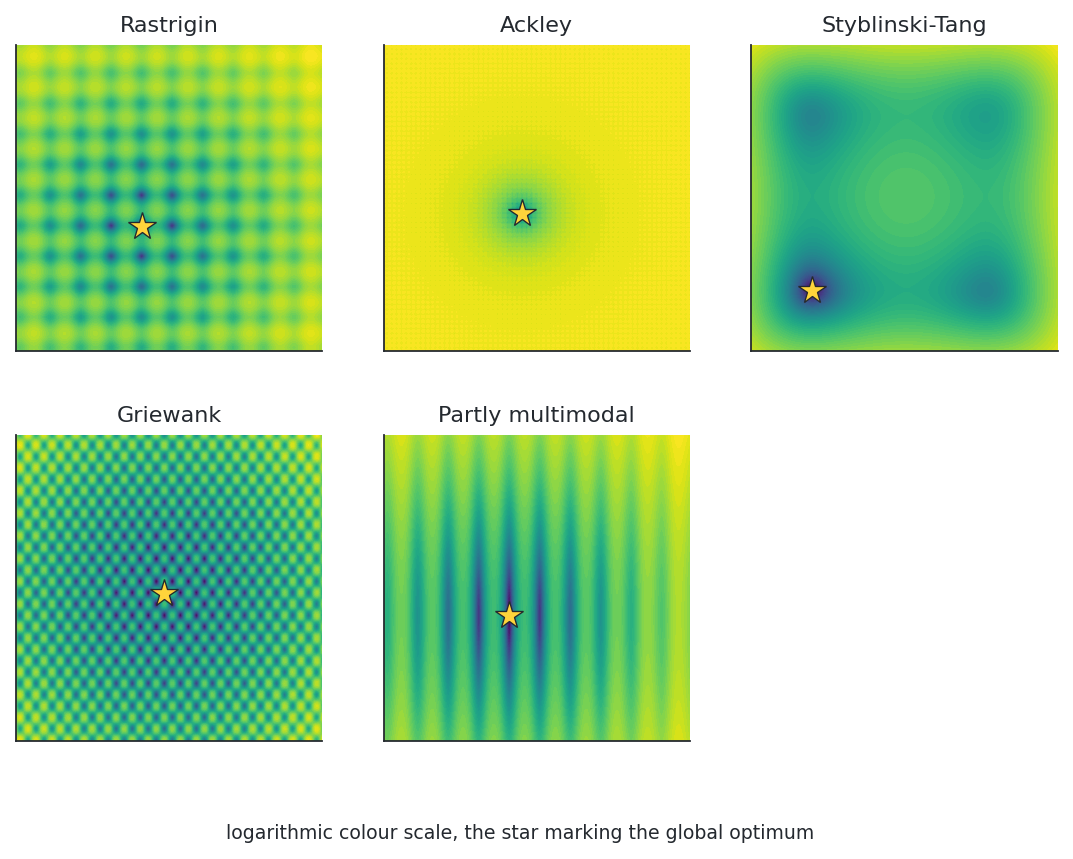
\includegraphics[width=\linewidth]{figures/problems.png}
  \caption{The five test problems in two dimensions.}
  \label{fig:problems}
\end{figure}

\subsection{Comparison with the enumeration of the boxes}\label{sec:enum}

The enumeration of the boxes, in which the sub-problem of every box is solved with
the same formulation, is used as a reference, so that the comparison concerns only
the exploration strategy. The results obtained for the Rastrigin function in two
dimensions with $10\times 10$ boxes and twenty starting points are given in
Table~\ref{tab:enum}. The
optimum is obtained by the outer approximation after the solution of 12 to 32\%
of the boxes, at a median cost of one quarter of that of the enumeration, and is
reached from nineteen of the twenty starting points.

The exploration of the configuration compared with the baselines
(Section~\ref{sec:baselines}), with the swept convexity, four probes and ten
subdivisions per variable, is illustrated for one starting point in
Fig.~\ref{fig:solve}. The four initial boxes are those of a design of
experiments including the box of the starting point. At the second iteration,
the trust regions of the three probes with radii below two contain the boxes
which differ from the incumbent in one component, and that of the fourth probe
contains every box. The box selected moves away from the incumbent as the
margin increases: the first probe selects an adjacent box, the second and the
third probes boxes two and six intervals away, and the fourth probe a box which
differs from the incumbent in both components. The global optimum is reached at
the sixth iteration, in the 22nd box solved.

\begin{table}[t]
  \centering
  \caption{Enumeration of the boxes and outer approximation for the Rastrigin
    function, $n=2$, $100$ boxes, twenty starting points: median objective
    value, and range over the starting points of the number of boxes solved and
    of the number of evaluations of the objective function.}
  \label{tab:enum}
  \begin{tabular}{lrrr}
    \toprule
    method & objective & boxes solved & evaluations \\
    \midrule
    enumeration          & $0.0$ & 100      & 1267 \\
    outer approximation  & $0.0$ & 12--32   & 158--412 \\
    \bottomrule
  \end{tabular}
\end{table}

\begin{figure}[t]
  \centering
  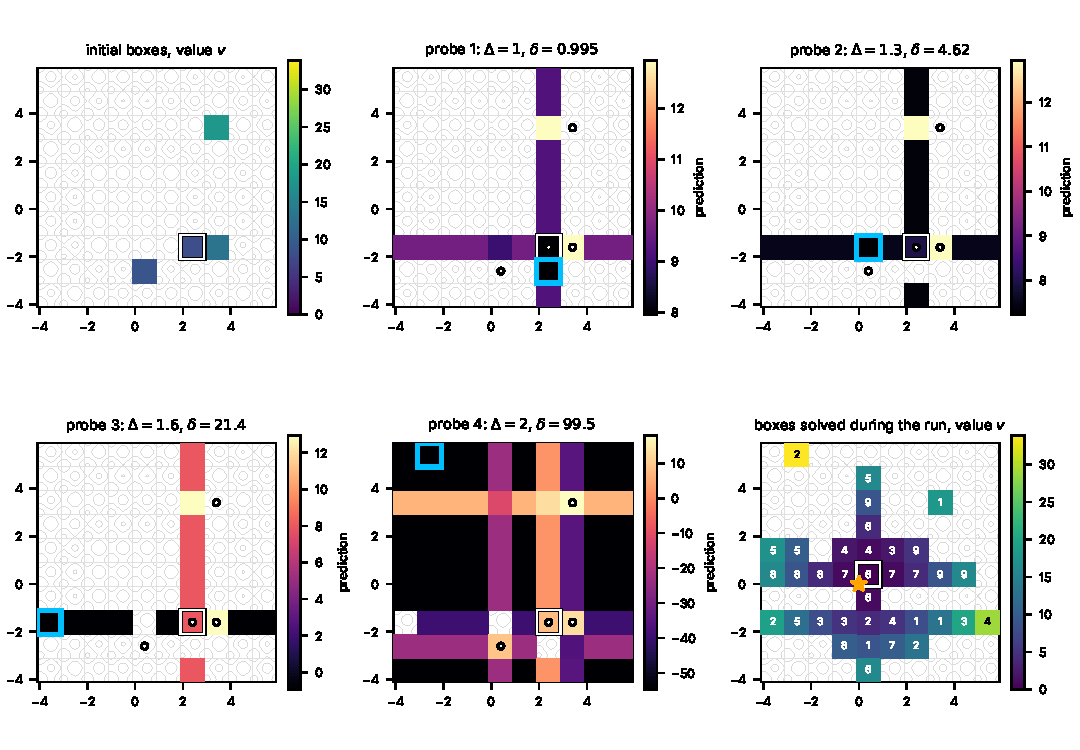
\includegraphics[width=\linewidth]{figures/exploration.pdf}
  \caption{Exploration of the method for the Rastrigin function, $n = 2$, swept
    convexity, four probes and $10 \times 10$ boxes, one starting point. Top
    left: boxes of the initial design of experiments, coloured by their value
    $v$, the incumbent being outlined in black. Next four panels: master problem
    of each probe at the second iteration, with its trust-region radius $\Delta$
    and its margin $\delta$; the boxes of its trust region are coloured by the
    prediction of the outer approximation, the boxes already solved are marked
    by dots, and the box selected is outlined in blue. The boxes selected by the
    previous probes of the iteration are excluded. Bottom right: boxes solved
    during the run, coloured by their value and numbered by iteration, the global
    optimum being marked by a star.}
  \label{fig:solve}
\end{figure}

\subsection{Safeguards and trust region}\label{sec:mechanisms}

The results of this section are detailed in Appendix~\ref{app:tuning}. The
useful range of the convexification constant becomes narrower as the dimension
increases: for the Rastrigin function, the median distance to the optimum is
zero for four of the five values tested in two dimensions, and for none of them
in five dimensions, where the optimum is reached from at most five starting
points out of twenty (Table~\ref{tab:constant}). With ten subdivisions in five
dimensions, it is reached from fifteen starting points with the adaptive repair
and four probes (Table~\ref{tab:density}); the adaptive repair is therefore used
by default, although this comparison also differs by the number of probes. Its
margin has to match the range of the objective function. On the Rastrigin
function in two dimensions, whose range is about $80$, the optimum is reached
with four probes from half of the starting points with a margin of $10$, and
from nineteen or twenty with a margin of $100$ or $300$
(Table~\ref{tab:margin}). On the Ackley function in five dimensions, whose range
is $14.5$, it is reached from one starting point with a margin of $100$, from
five or six with margins between $3$ and $30$, and from none with a margin of
$1$, only the last difference being significant
(Table~\ref{tab:margin-ackley}). This dependence motivates the swept convexity.

The ordinal trust region reaches the optimum as often as the Hamming distance
with a radius of one, at a higher cost (Table~\ref{tab:metric}). In five
dimensions, a radius of one reaches the optimum of the Rastrigin function
significantly less often than a radius of two, from seven starting points
against fifteen, and larger radii do not reach it more often; the median
distance to the optimum of the Ackley function increases with the radius, and
the optimum of the Styblinski--Tang function is reached from all starting
points with radii of three and five, against fifteen with a radius of two
(Table~\ref{tab:radius}). This radius is therefore a compromise for the problems
studied rather than a general rule.

\subsection{Variants of the method}\label{sec:variants}

Each variant differs from the configuration compared with the baselines, the
swept convexity with four probes, a ladder bounded by the spread of the
objective values and ten subdivisions per variable, by one setting, with one
exception: in five dimensions, the variants without a mark in
Table~\ref{tab:variants} use two subdivisions per variable, so that they differ
from the configuration also by the density. The configuration with a calibrated
margin $\delta = 100$ is included for comparison. The budget is $500n$
equivalent evaluations, and each variant is run on the four problems from the
twenty starting points of Section~\ref{sec:baselines}, so that it is paired with
the configuration by starting point and compared with it by the tests of that
section, the Holm correction running over the problems and the variants of each
dimension. The configuration was fixed before these runs, from a first study
with five starting points, and is kept unless a variant is clearly better: a
significantly higher success on some problem, or a larger area with a
confidence interval excluding zero, and a significantly lower success on none.
Sixteen probes with ten subdivisions per variable in five dimensions was not
run, a run taking several hours with fifty binary variables. The results are
given in Table~\ref{tab:variants} and the data profiles in
Fig.~\ref{fig:variants}.

\begin{table}[t]
  \centering
  \caption{Variants of the method, twenty starting points: area under the data
    profile, difference with the area of the configuration with its $95\%$
    bootstrap confidence interval, and problems on which the success differs
    significantly from that of the configuration (R: Rastrigin, A: Ackley, S:
    Styblinski--Tang, G: Griewank; $+$: more often, $-$: less often). In five
    dimensions, the variants without a mark use two subdivisions per variable,
    and $^1$ marks ten subdivisions per variable in both dimensions.}
  \label{tab:variants}
  \scriptsize
  \setlength{\tabcolsep}{2.5pt}
  \begin{tabular}{lrlrrll}
    \toprule
    & \multicolumn{3}{c}{$n = 2$} & \multicolumn{3}{c}{$n = 5$} \\
    \cmidrule(lr){2-4}\cmidrule(lr){5-7}
    variant & area & difference & success & area & difference & success \\
    \midrule
    swept, 4 probes, configuration       & 0.85 & \multicolumn{1}{c}{reference} & & 0.61 & \multicolumn{1}{c}{reference} & \\
    \quad 2 per variable                 & --- & & & 0.51 & $-0.10$ [$-0.14$, $-0.07$] & $-$R $-$A \\
    calibrated, margin 100               & 0.79 & $-0.06$ [$-0.09$, $-0.04$] &  & 0.49 & $-0.12$ [$-0.16$, $-0.08$] & $-$R $-$A \\
    swept, 8 probes                      & 0.86 & $+0.00$ [$-0.01$, $+0.01$] &  & 0.53 & $-0.09$ [$-0.12$, $-0.05$] & $-$R $-$A \\
    swept, 16 probes                     & 0.89 & $+0.04$ [$+0.01$, $+0.05$] &  & 0.49 & $-0.12$ [$-0.16$, $-0.09$] & $-$R $-$A \\
    swept, ladder up to 30               & 0.83 & $-0.02$ [$-0.05$, $+0.01$] &  & 0.48 & $-0.13$ [$-0.18$, $-0.09$] & $-$R $-$A \\
    swept, ladder up to 10               & 0.71 & $-0.15$ [$-0.21$, $-0.09$] & $-$A & 0.46 & $-0.15$ [$-0.19$, $-0.11$] & $-$R $-$A \\
    \quad 10 per variable$^1$              & --- & & & 0.58 & $-0.03$ [$-0.07$, $+0.00$] & $-$S \\
    swept, proposed density              & 0.53 & $-0.33$ [$-0.36$, $-0.29$] & $-$R $-$A & 0.18 & $-0.43$ [$-0.46$, $-0.40$] & $-$R $-$A \\
    \quad scans not charged              & 0.69 & $-0.16$ [$-0.19$, $-0.13$] & $-$A & 0.56 & $-0.05$ [$-0.09$, $-0.02$] & $-$A \\
    swept, 2 levels of 4                 & 0.77 & $-0.08$ [$-0.10$, $-0.07$] & $-$A & 0.43 & $-0.19$ [$-0.22$, $-0.15$] & $-$R $-$A $-$S \\
    swept, deep hierarchy                & 0.67 & $-0.18$ [$-0.20$, $-0.17$] & $-$R $-$A & 0.57 & $-0.04$ [$-0.07$, $-0.01$] & $-$R \\
    swept, Euclidean, diameter$^1$       & 0.84 & $-0.01$ [$-0.03$, $+0.01$] &  & 0.62 & $+0.01$ [$-0.02$, $+0.05$] &  \\
    swept, Euclidean, nearest box$^1$    & 0.78 & $-0.07$ [$-0.10$, $-0.04$] &  & 0.43 & $-0.19$ [$-0.22$, $-0.15$] & $-$S \\
    \bottomrule
  \end{tabular}
\end{table}

\begin{figure}[t]
  \centering
  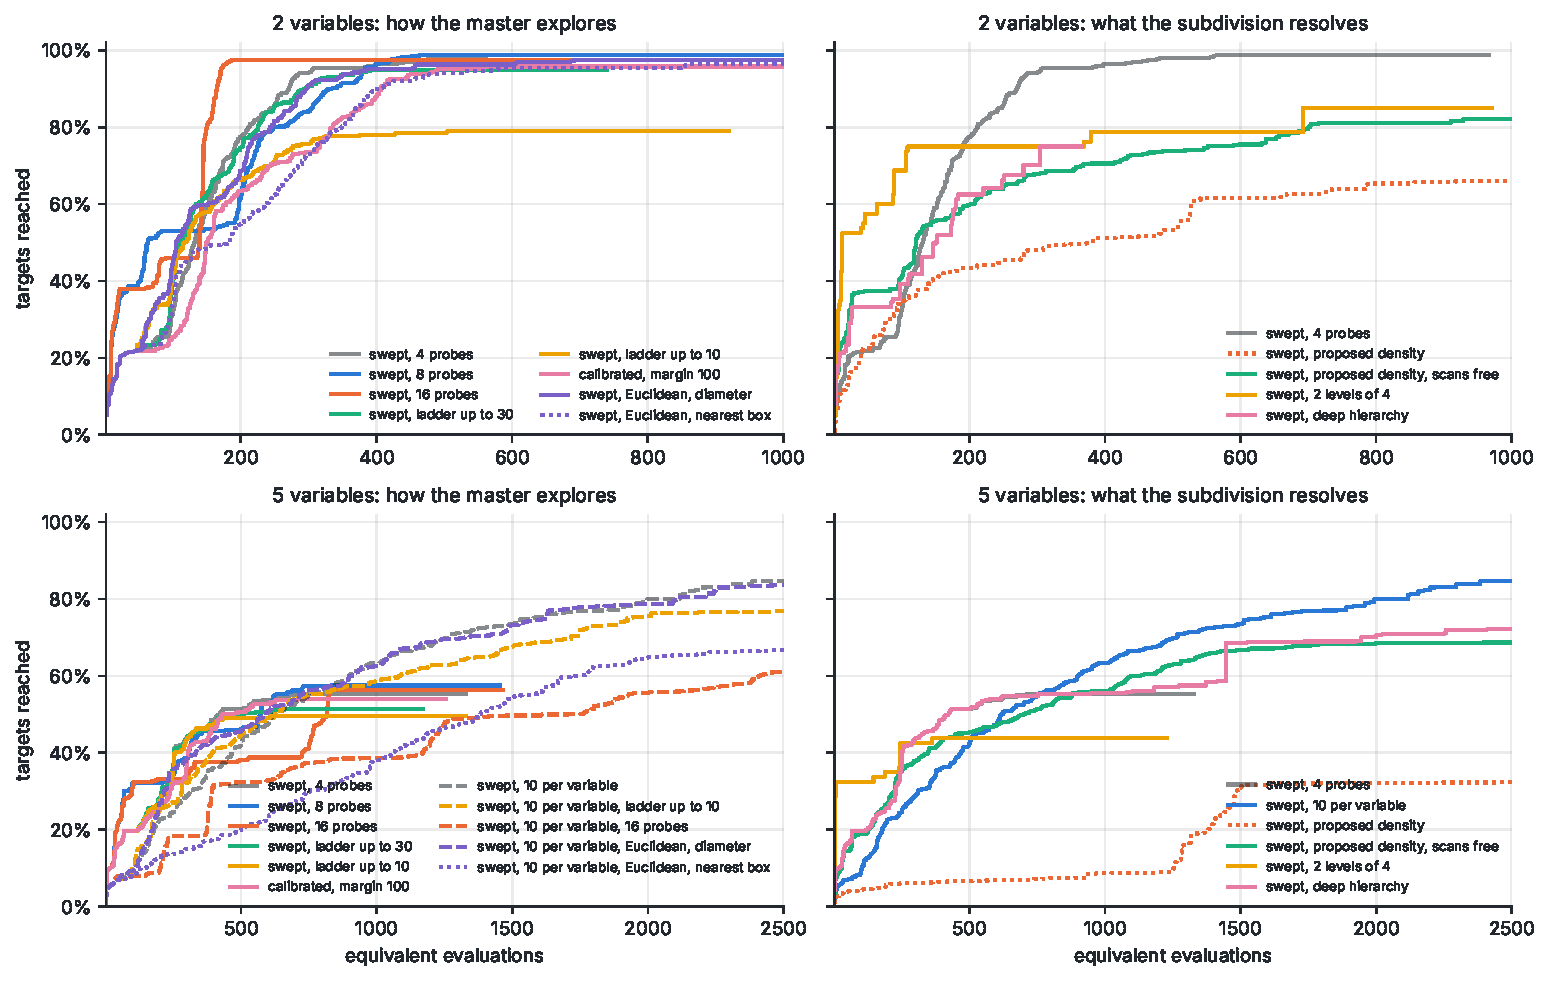
\includegraphics[width=\linewidth]{figures/variant_profiles.pdf}
  \caption{Data profiles of the variants of the method in two and five
    dimensions, twenty starting points. Dashed lines: variants with ten
    subdivisions per variable in five dimensions. Purple: Euclidean trust
    region, with the diameter schedule (solid or dashed) and around the nearest
    evaluated box (dotted).}
  \label{fig:variants}
\end{figure}

\paragraph{Number of probes.} In two dimensions, the area with sixteen probes is
larger than that of the configuration, by $0.04$ [$0.01$, $0.05$], with the same
success on every problem. Since this variant was selected among eleven on the
same starting points, it was run again with the configuration from twenty other
starting points: the difference of area is $0.045$ [$0.032$, $0.059$], and both
reach the optimum of the Rastrigin, Ackley and Styblinski--Tang functions from
all of them and that of the Griewank function from none. Sixteen probes
therefore reach the targets earlier in two dimensions without reaching the
optimum more often. With eight probes, the area is that of the configuration.

\paragraph{Upper bound of the ladder.} With an upper bound of $10$, the area
decreases by $0.15$ in both dimensions, and the optimum of the Ackley function in
two dimensions is reached less often. With an upper bound of $30$, no
difference is significant in two dimensions.

\paragraph{Calibrated margin.} The area of the calibrated configuration is
smaller than that of the swept configuration in two dimensions, by $0.06$, with
no significant difference of success.

\paragraph{Density.} In five dimensions, every variant which differs from the
configuration by the number of probes, the ladder or the margin, and uses two
subdivisions per variable, reaches the optimum of the Rastrigin and Ackley functions significantly
less often than the configuration, which reaches them from eleven and thirteen
starting points. The cost of the basin count used to estimate the density
exceeds the budget for most problems. Even when this cost is not counted, the
estimated density gives a smaller area than the fixed one in both dimensions,
since more than sixty subdivisions per variable are proposed for the Ackley
function (Section~\ref{sec:density-results}).

\paragraph{Extensions.} The multi-resolution encoding and the deep hierarchy
give smaller areas than the configuration in both dimensions.

\paragraph{Euclidean trust region.} With the diameter schedule, no difference
with the configuration is significant in either dimension. The union of balls
around the evaluated boxes gives smaller areas in both dimensions.

\paragraph{Choice of the configuration.} No variant is clearly better than the
configuration in five dimensions. In two dimensions, sixteen probes are, on the
area only; since this variant could not be run in five dimensions with ten
subdivisions per variable, the configuration with four probes is kept for the
comparison with the baselines, so that the same configuration is used in both
dimensions.

\subsection{Density of the subdivision}\label{sec:density-results}

The influence of the number $m$ of subdivisions per variable in five dimensions
is shown in Table~\ref{tab:density}, for the adaptive repair, a budget of $2500$
evaluations and twenty starting points. With about fifty sub-problems, ten
subdivisions per variable ($50$ binary variables, $10^5$ boxes) give the best
results for the Rastrigin function, and sixteen subdivisions ($80$ binary
variables) significantly worse results, in agreement with the upper bound of
Section~\ref{sec:density}.

\begin{table}[t]
  \centering
  \caption{Influence of the number $m$ of subdivisions per variable, $n=5$:
    median distance to the optimum $\cdot$ median cost $\cdot$ number of starting
    points out of twenty from which the optimum is reached (when non-zero).
    $\dagger$ Median run stopped by the budget, for which the distance is an
    upper bound.}
  \label{tab:density}
  \small
  \begin{tabular}{rrrllll}
    \toprule
    $m$ & bin. & boxes & Rastrigin & Ackley & Styblinski--Tang & Griewank \\
    \midrule
    2  & 10  & $32$            & 4.98 $\cdot$ 866                & 14.43 $\cdot$ 674                    & 0.00 $\cdot$ 481 $\cdot$ 16/20  & 0.06 $\cdot$ 1015 \\
    4  & 20  & $10^3$          & 6.70 $\cdot$ 801                & 12.63 $\cdot$ 1270                   & 0.00 $\cdot$ 749 $\cdot$ 19/20  & 0.22 $\cdot$ 1349 \\
    10 & 50  & $10^5$          & 0.00 $\cdot$ 1757 $\cdot$ 15/20 & 6.30 $\cdot$ 2500$\dagger$ $\cdot$ 1/20 & 0.00 $\cdot$ 582 $\cdot$ 15/20  & 0.05 $\cdot$ 2500$\dagger$ \\
    16 & 80  & $10^6$          & 1.99 $\cdot$ 1780 $\cdot$ 1/20  & 5.53 $\cdot$ 2500$\dagger$ $\cdot$ 3/20 & 0.13 $\cdot$ 864 $\cdot$ 10/20  & 0.06 $\cdot$ 2500$\dagger$ \\
    24 & 120 & $8\cdot 10^6$   & 2.86 $\cdot$ 1834 $\cdot$ 1/20  & 8.90 $\cdot$ 2500$\dagger$           & 0.13 $\cdot$ 1122 $\cdot$ 8/20  & 0.08 $\cdot$ 2500$\dagger$ \\
    \bottomrule
  \end{tabular}
\end{table}

With ten subdivisions per variable, i.e. $10^5$ boxes and $50$ binary variables,
the optimum of the Rastrigin function in five dimensions is reached from
fifteen starting points out of twenty with a median of about $1750$ evaluations,
and from eleven with the swept convexity of the configuration compared in
Section~\ref{sec:baselines}, whereas it is not reached by any of the baselines
with the budgets considered. With sixteen and twenty-four subdivisions, the runs
terminate on their own criterion at a similar cost but reach the optimum from
one starting point, since eighty binary variables cannot be identified with
about fifty cuts. The optimum of the Styblinski--Tang function, which has two
basins per variable, is reached from fifteen to nineteen starting points with
two to ten subdivisions, and significantly less often with twenty-four. Both
bounds of Section~\ref{sec:density} are therefore observed. For the Ackley and
Griewank functions, the optimum is reached from at most three starting points
with any density, and most runs with ten or more subdivisions were stopped by
the budget, so that the corresponding results only rank the progress made within
the budget.

\paragraph{Estimated density.} For the results of Table~\ref{tab:proposed}, each
problem is given four times the budget corresponding to its estimated density, so
that all runs terminate on their own stopping criterion. For the Rastrigin and
Styblinski--Tang functions, the estimated densities are ten and two subdivisions
per variable, which reach the optimum from fifteen and sixteen starting points
out of twenty. For the partly multimodal function, the three unimodal components
are not subdivided, and the optimum is reached from all starting points with a
median of $990$ evaluations, against none with two subdivisions of the five
variables (Table~\ref{tab:partial}). For the Ackley function, the basin count does
not converge. The oscillations of this function are indeed about one unit apart
over a range of sixty-four, but the global basin, and not the oscillations, has
to be resolved, and the estimate is correctly reported as unresolved before the
run.

The scans require between $1250$ and $12\,525$ evaluations for the problems whose
count converged, and $25\,350$ for the Ackley function (Table~\ref{tab:proposed}).
These evaluations are not included in the cost of the runs, and the estimation of
the density is therefore affordable only when the evaluation of the objective
function is inexpensive compared with the solution of a sub-problem.

\begin{table}[t]
  \centering
  \caption{Results obtained with the estimated density and the calibrated margin,
    $n = 5$, twenty starting points and a budget equal to four times the
    predicted cost: median distance, median cost and number of starting points
    from which the optimum is reached. The cost of the
    scans, given in the last column, is not included in the cost of the runs.}
  \label{tab:proposed}
  \small
  \begin{tabular}{llrrrrr}
    \toprule
    problem & proposed $m$ & binaries & distance & cost & reached & scans \\
    \midrule
    Rastrigin         & $10^{\times 5}$ & 50 & 0.00 & 1757 & 15/20 & 12\,525 \\
    Styblinski--Tang  & $2^{\times 5}$  & 10 & 0.00 & 481  & 16/20 & 1250 \\
    partly multimodal & 10, 10, 1, 1, 1 & 23 & 0.00 & 990  & 20/20 & 6100 \\
    Griewank          & 19, 13, 11, 7, 9 & 59 & 0.034 & 3631 & 0/20 & 12\,525 \\
    Ackley            & $63^{\times 5}$, unresolved & 314 & 14.72 & 3170 & 0/20 & 25\,350 \\
    \bottomrule
  \end{tabular}
\end{table}

\subsection{Swept and calibrated convexity}\label{sec:sweep-results}

Fixed and swept convexity values are compared in Table~\ref{tab:sweep} for the
Rastrigin and Ackley functions in two dimensions, whose ranges differ by a factor
of four, with ten subdivisions per variable, a budget of $1000$ evaluations and
twenty starting points. With a margin of $10$, the optimum of both problems is
reached from half of the starting points, significantly less often than with
either swept configuration. With a margin of $100$, it is reached from nineteen
and seventeen starting points, and with the swept configurations from all or
all but one, including the unbounded one, for which no convexity value is
specified; these differences are not significant. The
additional values of the ladder require mixed-integer solutions but no
evaluations of the objective, so that the costs of the swept and calibrated
configurations are similar. These results concern two problems which were also
used to select the headroom factor, and a broader comparison is given in
Table~\ref{tab:variants}.

\begin{table}[t]
  \centering
  \caption{Fixed and swept convexity, $n = 2$, twenty starting points: median
    distance $\cdot$ median cost $\cdot$ number of starting points from which the
    optimum is reached.}
  \label{tab:sweep}
  \begin{tabular}{lll}
    \toprule
    convexity & Rastrigin (range $\approx 80$) & Ackley (range $\approx 22$) \\
    \midrule
    fixed, margin 10                   & 0.497 $\cdot$ 183 $\cdot$ 10/20 & 3.814 $\cdot$ 270 $\cdot$ 10/20 \\
    fixed, margin 100                  & 0.000 $\cdot$ 541 $\cdot$ 19/20 & 0.000 $\cdot$ 528 $\cdot$ 17/20 \\
    sweep, $\delta_{\max} = 100$       & 0.000 $\cdot$ 539 $\cdot$ 20/20 & 0.000 $\cdot$ 517 $\cdot$ 19/20 \\
    sweep, unbounded                   & 0.000 $\cdot$ 540 $\cdot$ 20/20 & 0.000 $\cdot$ 491 $\cdot$ 20/20 \\
    \bottomrule
  \end{tabular}
\end{table}

The swept convexity does not give better results than the calibrated margin in
all cases. In Table~\ref{tab:sweep-density}, the comparison is repeated in five
dimensions with the densities estimated by the basin count, so that neither a
margin nor a density is specified for the swept runs. With the swept convexity,
the optimum of the Ackley function with ten subdivisions is reached from
thirteen starting points out of twenty, significantly more often than from the
four of the calibrated margin, which exceeds the range of this function. The
optimum of the Griewank function is reached by neither, the median distance
being $0.012$ with the swept convexity and $0.034$ with the calibrated margin.
For the Rastrigin function, however, the optimum is reached from eleven starting
points with the swept convexity and from fifteen with the calibrated margin, a
difference which is not significant. It should be noted that the calibrated
margin represents $54\%$ of the range of the Rastrigin function and was
calibrated on this function.

\begin{table}[t]
  \centering
  \caption{Swept and calibrated convexity with the estimated densities, $n = 5$,
    twenty starting points: median distance $\cdot$ median cost $\cdot$ number of
    starting points from which the optimum is reached.}
  \label{tab:sweep-density}
  \small
  \begin{tabular}{llll}
    \toprule
    problem & density & swept & calibrated, $\delta = 100$ \\
    \midrule
    Styblinski--Tang  & $2^{\times 5}$     & 0.000 $\cdot$ 601 $\cdot$ 19/20  & 0.000 $\cdot$ 481 $\cdot$ 16/20 \\
    partly multimodal & 10, 10, 1, 1, 1    & 0.000 $\cdot$ 848 $\cdot$ 20/20  & 0.000 $\cdot$ 990 $\cdot$ 20/20 \\
    Ackley            & $10^{\times 5}$    & 0.000 $\cdot$ 2662 $\cdot$ 13/20 & 4.945 $\cdot$ 2620 $\cdot$ 4/20 \\
    Griewank          & 19, 13, 11, 7, 9   & 0.012 $\cdot$ 3189 $\cdot$ 0/20  & 0.034 $\cdot$ 3631 $\cdot$ 0/20 \\
    Ackley            & $63^{\times 5}$    & 8.735 $\cdot$ 3341 $\cdot$ 0/20  & 14.72 $\cdot$ 3170 $\cdot$ 0/20 \\
    Rastrigin         & $10^{\times 5}$    & 0.000 $\cdot$ 1756 $\cdot$ 11/20 & 0.000 $\cdot$ 1757 $\cdot$ 15/20 \\
    \bottomrule
  \end{tabular}
\end{table}

\subsection{Extensions}\label{sec:extensions-results}

The extensions of Section~\ref{sec:extensions} were evaluated in five dimensions
with a budget of $2500$ equivalent evaluations and the calibrated margin. The
detailed results are given in Appendix~\ref{app:extensions}.

\paragraph{Partial subdivision.} For the partly multimodal function, the optimum
is reached from all starting points when only the two variables of the Rastrigin
function are divided into ten intervals, and from none of them with a coarse
subdivision of the five variables (Table~\ref{tab:partial}). A subdivision which
does not correspond exactly to the multimodal variables can also succeed:
dividing three variables into four intervals ($12$ binary variables) reaches the
optimum from seventeen starting points with a median of $758$ evaluations,
against twenty with $990$ evaluations when two variables are divided into ten
($20$ binary variables), a difference of success which is not significant. The
cost depends mainly on the number of binary variables.

\paragraph{Multi-resolution encoding.} With two levels of four intervals, a
resolution of sixteen intervals per variable is obtained with forty binary
variables instead of eighty (Table~\ref{tab:multires}). Compared with sixteen
subdivisions with the standard encoding, the results are similar for the
Rastrigin function and worse for the Ackley and Styblinski--Tang functions, the
optimum of the latter being reached from two starting points out of twenty
instead of ten. For the same resolution and number of binary variables, two
levels of four intervals give smaller median distances than four levels of two
intervals for the three functions. This is consistent with the additive cut
model, which becomes less accurate as the number of levels increases.

\paragraph{Hierarchies.} With the deep hierarchy, in which every variable is
divided into two intervals at each of four levels, the optimum of the Ackley
function in five dimensions is reached from twelve starting points out of
twenty, against one with ten subdivisions per variable, and the runs terminate
on their own criterion. For the Rastrigin function, the results are worse than
with a single subdivision, and for the Styblinski--Tang function, the optimum is
reached as often as with two subdivisions per variable, at three times the cost
(Table~\ref{tab:hierarchies}). The best-first search, which is the only variant
able to revise the choice of a box, gives the worst results for the Rastrigin function. A budget which provides fifty
cuts to a single cut model provides only five cuts to each of ten models, which
are then not sufficiently determined to rank the boxes.

\paragraph{Influence of the budget.} Since several of these comparisons involve
runs stopped by the budget, the most sensitive one was repeated with two and four
times the budget (Table~\ref{tab:budget}). The optimum of the Ackley function is
then reached with ten subdivisions per variable from four starting points out of
twenty instead of one, and with the deep hierarchy from twelve in both cases, a
difference which remains significant. Beyond twice the budget, the results are
unchanged, since both configurations terminate on their own stopping criteria.

\subsection{Comparison with the baselines}\label{sec:baselines}

The same configuration of the method is used in both dimensions for the
comparison: the swept convexity with four probes and ten subdivisions per
variable, the density being the one selected on these problems
(Section~\ref{sec:protocol}). Each method is run from twenty starting points per
problem, the same for all methods. The results obtained for each problem are
given in Table~\ref{tab:baselines}, the paired tests in Table~\ref{tab:tests},
and the data profiles in Table~\ref{tab:profiles} and Fig.~\ref{fig:profiles}.
EGO is run with a budget of $500$ evaluations, which is the largest budget
compatible with the cost of its surrogate model.

The two methods of each comparison are paired by starting point. The success,
i.e. a distance to the optimum below the tolerance of the benchmark, is compared
by the exact McNemar test, a binomial test on the starting points from which
exactly one of the two methods reaches the optimum, and the final distance by
the Wilcoxon signed-rank test. The $p$-values of each dimension are corrected by
the Holm procedure over the four problems and the five baselines, and a
difference is called significant below $0.05$ after correction. The area under
the data profile is computed against the targets of Section~\ref{sec:protocol},
which were generated from the runs of the first five starting points, and its difference with each baseline is given with a $95\%$ confidence interval
obtained by a bootstrap over the starting points, paired across methods. These
two measures were fixed before the runs were made. DIRECT, which uses no
starting point, gives the same run from every starting point, so that the
comparison with DIRECT is a comparison with a single result and its interval
reflects only the variability of the method.

\begin{table}[t]
  \centering
  \caption{Comparison of the method, swept with ten subdivisions per variable,
    with the baselines, $500n$ equivalent evaluations, twenty starting points:
    median distance $\cdot$ median cost $\cdot$ number of starting points from
    which the optimum is reached. $\ddagger$ EGO is run with $500$
    evaluations.}
  \label{tab:baselines}
  \scriptsize
  \setlength{\tabcolsep}{2pt}
  \begin{tabular}{lrllllll}
    \toprule
    problem & $n$ & box subdivision & multistart & CMA-ES & DIRECT & tunneling & EGO$\ddagger$ \\
    \midrule
    Rastrigin        & 2 & 0.00 $\cdot$ 538 $\cdot$ 20   & 1.00 $\cdot$ 1000 $\cdot$ 9 & 1.00 $\cdot$ 625 $\cdot$ 4   & 0.00 $\cdot$ 649 $\cdot$ 20  & 1.99 $\cdot$ 1000 $\cdot$ 0  & 0.00 $\cdot$ 500 $\cdot$ 12 \\
    Ackley           & 2 & 0.00 $\cdot$ 575 $\cdot$ 20   & 0.00 $\cdot$ 1000 $\cdot$ 12 & 0.00 $\cdot$ 751 $\cdot$ 20 & 0.00 $\cdot$ 417 $\cdot$ 20  & 0.00 $\cdot$ 1000 $\cdot$ 19 & 0.32 $\cdot$ 500 $\cdot$ 0 \\
    Styblinski--Tang & 2 & 0.00 $\cdot$ 348 $\cdot$ 20   & 0.00 $\cdot$ 1000 $\cdot$ 20 & 0.00 $\cdot$ 532 $\cdot$ 12 & 0.00 $\cdot$ 1011 $\cdot$ 20 & 0.00 $\cdot$ 1000 $\cdot$ 20 & 0.00 $\cdot$ 500 $\cdot$ 20 \\
    Griewank         & 2 & 0.007 $\cdot$ 628 $\cdot$ 0  & 0.027 $\cdot$ 1000 $\cdot$ 1 & 0.047 $\cdot$ 766 $\cdot$ 1 & 0.007 $\cdot$ 1011 $\cdot$ 0 & 0.027 $\cdot$ 1000 $\cdot$ 1 & 0.024 $\cdot$ 500 $\cdot$ 2 \\
    Rastrigin        & 5 & 0.00 $\cdot$ 1756 $\cdot$ 11  & 5.97 $\cdot$ 2500 $\cdot$ 0 & 4.97 $\cdot$ 1749 $\cdot$ 0  & 4.98 $\cdot$ 461 $\cdot$ 0   & 4.97 $\cdot$ 2500 $\cdot$ 0  & 3.99 $\cdot$ 500 $\cdot$ 0 \\
    Ackley           & 5 & 0.00 $\cdot$ 2500 $\cdot$ 13  & 9.28 $\cdot$ 2500 $\cdot$ 0 & 0.00 $\cdot$ 1921 $\cdot$ 19 & 0.11 $\cdot$ 353 $\cdot$ 0   & 2.32 $\cdot$ 2500 $\cdot$ 4  & 1.40 $\cdot$ 500 $\cdot$ 0 \\
    Styblinski--Tang & 5 & 0.00 $\cdot$ 842 $\cdot$ 18   & 0.00 $\cdot$ 2326 $\cdot$ 20 & 14.14 $\cdot$ 1409 $\cdot$ 8 & 0.00 $\cdot$ 2505 $\cdot$ 20 & 0.00 $\cdot$ 2500 $\cdot$ 15 & 0.00 $\cdot$ 500 $\cdot$ 20 \\
    Griewank         & 5 & 0.027 $\cdot$ 2200 $\cdot$ 0 & 0.046 $\cdot$ 2500 $\cdot$ 0 & 0.028 $\cdot$ 1681 $\cdot$ 0 & 0.011 $\cdot$ 397 $\cdot$ 0 & 0.070 $\cdot$ 2500 $\cdot$ 0 & 0.064 $\cdot$ 500 $\cdot$ 0 \\
    \bottomrule
  \end{tabular}
\end{table}

\begin{table}[t]
  \centering
  \caption{Paired comparison of the success, twenty starting points: number of
    starting points from which only the method reaches the optimum $-$ number
    from which only the baseline does, with the $p$-value of the exact McNemar
    test after Holm correction. Bold: significant at $0.05$. ---: no
    discordant starting point.}
  \label{tab:tests}
  \scriptsize
  \setlength{\tabcolsep}{3pt}
  \begin{tabular}{lrlllll}
    \toprule
    problem & $n$ & multistart & CMA-ES & DIRECT & tunneling & EGO \\
    \midrule
    Rastrigin        & 2 & \textbf{11$-$0}, 0.017 & \textbf{16$-$0}, 0.001 & ---               & \textbf{20$-$0}, $<$0.001 & 8$-$0, 0.125 \\
    Ackley           & 2 & 8$-$0, 0.125           & ---                    & ---               & 1$-$0, 1.000              & \textbf{20$-$0}, $<$0.001 \\
    Styblinski--Tang & 2 & ---                    & 8$-$0, 0.125           & ---               & ---                       & --- \\
    Griewank         & 2 & 0$-$1, 1.000           & 0$-$1, 1.000           & ---               & 0$-$1, 1.000              & 0$-$2, 1.000 \\
    Rastrigin        & 5 & \textbf{11$-$0}, 0.017 & \textbf{11$-$0}, 0.017 & \textbf{11$-$0}, 0.017 & \textbf{11$-$0}, 0.017 & \textbf{11$-$0}, 0.017 \\
    Ackley           & 5 & \textbf{13$-$0}, 0.005 & 0$-$6, 0.312           & \textbf{13$-$0}, 0.005 & 11$-$2, 0.247         & \textbf{13$-$0}, 0.005 \\
    Styblinski--Tang & 5 & 0$-$2, 1.000           & 11$-$1, 0.076          & 0$-$2, 1.000      & 4$-$1, 1.000              & 0$-$2, 1.000 \\
    Griewank         & 5 & ---                    & ---                    & ---               & ---                       & --- \\
    \bottomrule
  \end{tabular}
\end{table}

\begin{table}[t]
  \centering
  \caption{Area under the data profile and fraction of the targets reached at a
    tenth, a quarter and a half of the budget and at the end of the budget,
    twenty starting points, and difference of the area of the method with that
    of each baseline, with its $95\%$ bootstrap confidence interval.
    $\ddagger$ Value at the end of the budget of EGO, i.e. $500$ evaluations,
    which in five dimensions is less than a quarter of the budget of the other
    methods; no area is given for EGO.}
  \label{tab:profiles}
  \scriptsize
  \setlength{\tabcolsep}{3pt}
  \begin{tabular}{rlrrrrrl}
    \toprule
    $n$ & method & area & $\tfrac1{10}$ & $\tfrac14$ & $\tfrac12$ & end & difference \\
    \midrule
    2 & box subdivision      & 0.85 & 32\% & 86\% & 98\% & 99\% & \\
    2 & multistart           & 0.73 & 46\% & 67\% & 79\% & 90\% & $+0.12$ [$+0.09$, $+0.15$] \\
    2 & CMA-ES               & 0.72 & 52\% & 69\% & 79\% & 80\% & $+0.13$ [$+0.08$, $+0.19$] \\
    2 & DIRECT               & 0.90 & 69\% & 84\% & 99\% & 99\% & $-0.04$ [$-0.06$, $-0.03$] \\
    2 & tunneling            & 0.74 & 55\% & 68\% & 79\% & 87\% & $+0.11$ [$+0.07$, $+0.15$] \\
    2 & EGO, 500 evaluations & ---  & 73\% & 82\% & 85\% & 85\%$\ddagger$ & \\
    \midrule
    5 & box subdivision      & 0.61 & 25\% & 51\% & 70\% & 85\% & \\
    5 & multistart           & 0.52 & 40\% & 50\% & 56\% & 61\% & $+0.09$ [$+0.05$, $+0.13$] \\
    5 & CMA-ES               & 0.64 & 42\% & 61\% & 72\% & 74\% & $-0.02$ [$-0.06$, $+0.02$] \\
    5 & DIRECT               & 0.76 & 75\% & 79\% & 79\% & 79\% & $-0.15$ [$-0.18$, $-0.11$] \\
    5 & tunneling            & 0.65 & 40\% & 61\% & 71\% & 76\% & $-0.03$ [$-0.07$, $+0.01$] \\
    5 & EGO, 500 evaluations & ---  & 61\% & ---  & ---  & 69\%$\ddagger$ & \\
    \bottomrule
  \end{tabular}
\end{table}

\begin{figure}[t]
  \centering
  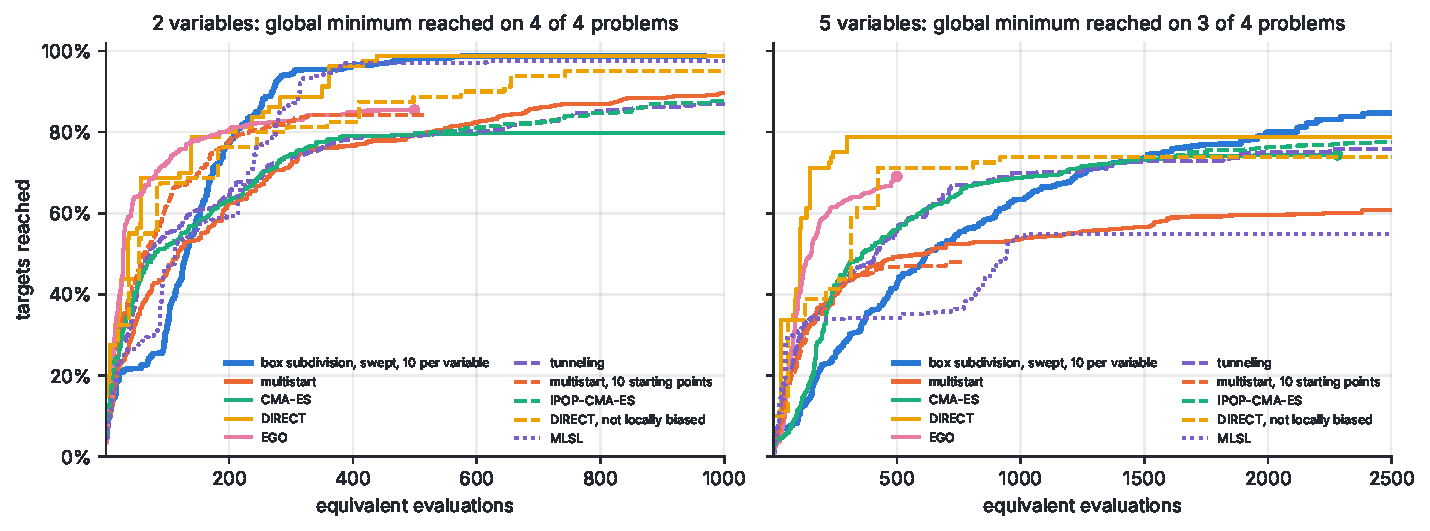
\includegraphics[width=\linewidth]{figures/data_profiles.pdf}
  \caption{Data profiles of the method, swept with ten subdivisions per
    variable, and of the baselines, twenty starting points. The end of the
    budget of EGO is marked on its curve. Tunneling is dashed.}
  \label{fig:profiles}
\end{figure}

In five dimensions, the optimum of the Rastrigin function is reached by the
method from eleven starting points out of twenty, and by none of the baselines
from any starting point; the difference is significant against each baseline.
That of the Ackley function is reached from thirteen starting points, against
none for the multistart algorithm, DIRECT and EGO, with significant
differences, four for tunneling and nineteen for CMA-ES; these last two
differences are not significant. For the Styblinski--Tang function, the method
reaches the optimum from eighteen starting points, CMA-ES from eight, and the
other baselines from fifteen to twenty, with no significant difference. In two
dimensions, the method reaches the optimum of the Rastrigin, Ackley and
Styblinski--Tang functions from all starting points, as DIRECT does, and the
difference is significant on the Rastrigin function against the multistart
algorithm, CMA-ES and tunneling, and on the Ackley function against EGO. The
optimum of the Griewank function is reached from at most two starting points by
any method in either dimension. The final distances to it are smaller with the
method than with the multistart algorithm, CMA-ES, tunneling and EGO in two
dimensions, and larger than with DIRECT in five dimensions ($0.027$ against
$0.011$), these differences being significant. For the Ackley function in five
dimensions, the final distances are significantly smaller with CMA-ES. The other
significant differences of final distance found by the signed-rank test either
agree with those of the success or are below $10^{-4}$ on problems whose optimum
is reached by both methods, and are not discussed.

The area of the method is larger than those of the multistart algorithm, CMA-ES
and tunneling in two dimensions, and than that of the multistart algorithm in
five dimensions. It is smaller than that of DIRECT in both dimensions, by $0.04$
and $0.15$: DIRECT reaches the targets earlier, while the method reaches the
optimum from as many starting points in two dimensions, and in five dimensions
from more starting points for the Rastrigin and Ackley functions and from two
fewer for the Styblinski--Tang function. In five dimensions, the confidence intervals of the differences with
CMA-ES and tunneling contain zero. The method reaches $25\%$ of the targets at a
tenth of the budget, the lowest fraction of all methods in both dimensions, and
$85\%$ at the end of the budget in five dimensions, the largest fraction.

\subsection{Comparison with a budget of 500 evaluations}\label{sec:small}

A budget of $500n$ evaluations is large for industrial applications, and does not
allow the use of Bayesian optimization, whose computational cost grows cubically
with the number of samples. All methods are therefore compared in
Table~\ref{tab:small} with a budget of $500$ evaluations, from the twenty
starting points of Section~\ref{sec:baselines} and by the same paired tests, the
method being used in the configuration of that section, swept with ten
subdivisions per variable.

\begin{table}[t]
  \centering
  \caption{Budget of $500$ evaluations, twenty starting points: median distance
    to the optimum $\cdot$ number of starting points from which the optimum is
    reached, and median cost when it is smaller than the budget.}
  \label{tab:small}
  \scriptsize
  \setlength{\tabcolsep}{3pt}
  \begin{tabular}{lrllllll}
    \toprule
    problem & $n$ & box subdivision & multistart & CMA-ES & DIRECT & EGO & tunneling \\
    \midrule
    Rastrigin        & 2 & 0.00 $\cdot$ 20 & 1.00 $\cdot$ 6 & 1.00 $\cdot$ 4 & 0.00 $\cdot$ 20 & 0.00 $\cdot$ 12 & 1.99 $\cdot$ 0 \\
    Ackley           & 2 & 0.00 $\cdot$ 19 & 3.57 $\cdot$ 2 & 0.00 $\cdot$ 20 & 0.00 $\cdot$ 20 $\cdot$ 417 & 0.32 $\cdot$ 0 & 0.00 $\cdot$ 13 \\
    Styblinski--Tang & 2 & 0.00 $\cdot$ 20 $\cdot$ 348 & 0.00 $\cdot$ 20 & 0.00 $\cdot$ 12 & 0.00 $\cdot$ 20 & 0.00 $\cdot$ 20 & 0.00 $\cdot$ 20 \\
    Griewank         & 2 & 0.007 $\cdot$ 0 & 0.053 $\cdot$ 1 & 0.052 $\cdot$ 1 & 0.009 $\cdot$ 0 & 0.024 $\cdot$ 2 & 0.027 $\cdot$ 0 \\
    Rastrigin        & 5 & 6.47 $\cdot$ 0 & 9.95 $\cdot$ 0 & 11.20 $\cdot$ 0 & 4.98 $\cdot$ 0 $\cdot$ 461 & 3.99 $\cdot$ 0 & 4.97 $\cdot$ 0 \\
    Ackley           & 5 & 16.70 $\cdot$ 0 & 16.30 $\cdot$ 0 & 0.05 $\cdot$ 0 & 0.11 $\cdot$ 0 $\cdot$ 353 & 1.40 $\cdot$ 0 & 6.09 $\cdot$ 2 \\
    Styblinski--Tang & 5 & 6.03 $\cdot$ 10 & 7.15 $\cdot$ 9 & 14.14 $\cdot$ 6 & 0.00 $\cdot$ 20 & 0.00 $\cdot$ 20 & 14.14 $\cdot$ 7 \\
    Griewank         & 5 & 0.440 $\cdot$ 0 & 0.097 $\cdot$ 0 & 0.276 $\cdot$ 0 & 0.011 $\cdot$ 0 $\cdot$ 397 & 0.064 $\cdot$ 0 & 0.221 $\cdot$ 0 \\
    \bottomrule
  \end{tabular}
\end{table}

In two dimensions, the method reaches the optimum of the Rastrigin, Ackley and
Styblinski--Tang functions from twenty, nineteen and twenty starting points,
significantly more often than the multistart algorithm on the Rastrigin and
Ackley functions, than CMA-ES and tunneling on the Rastrigin function, and than
EGO on the Ackley function. In five dimensions, the optimum of the Rastrigin
function is reached by no method; the median distance is $3.99$ for EGO,
$4.97$ for tunneling, $4.98$ for DIRECT and $6.47$ for the method, and no
difference between the method and a baseline is significant. The fifty binary
variables of the method cannot be identified with the cuts of $500$
evaluations: all its runs are stopped by the budget, the optimum of the
Styblinski--Tang function is reached from ten starting points, significantly
fewer than the twenty of DIRECT and EGO, and its final distances to the optimum
of the Ackley function are significantly larger than those of CMA-ES, DIRECT,
EGO and tunneling, and to that of the Griewank function than those of the
multistart algorithm, DIRECT and EGO.

\subsection{Application to topology optimization}\label{sec:cantilever}

The short cantilever problem of the generalized geometry projection (GGP)
\citep{coniglio2020,ggpcode} is a constrained problem with adjoint sensitivities.
The structure is described by $18$ bars, each defined by the position of its
centre, its angle, length, thickness and density, which gives $108$ design
variables, and the compliance $C$ is minimized subject to a volume fraction of
$0.4$ on a mesh of $60\times 30$ elements. The settings of the reference MATLAB
implementation with the moving node approach are used: a cubic characteristic
function, a lower-bound Kreisselmeier--Steinhauser aggregation
\citep{kreisselmeier1979} with $k_a = 10$ followed by a smooth saturation, a
penalization exponent $p = 3$, bounds of $[-2\pi, 2\pi]$ on the angles, the
objective function $\log(C+1)$, and MMA \citep{svanberg1987} with a move limit of
$0.01$.

The position and the angle of every bar are divided into ten intervals, which
gives $54$ subdivided variables and $540$ binary variables, while the length, the
thickness and the density of the bars remain continuous variables of every
sub-problem. The convexity is swept, nine boxes are proposed at each iteration of
the master problem and solved in parallel, and each sub-problem is solved by MMA
with at most $1800$ iterations. For comparison, the same problem is solved by MMA
from $63$ initial designs, one for each box solved by the method, namely the
reference initial design and $62$ designs whose bar positions and angles are
drawn uniformly within the bounds. The problem is also solved by the classic
tunneling method with the volume constraint kept in the tunneling phase
\citep{levy1985,levygomez1985}, with the same budget as the box-subdivision
method. The minimizations and the tunneling phases are solved by MMA with the
same settings, the first minimization being started from the reference initial
design, and four tunneling searches from the same minimizer are run in
parallel. This run was performed on a NumPy port of the reference MATLAB code,
which reproduces the solution obtained from the reference initial design
(Table~\ref{tab:cantilever}), and not on the implementation used for the other
methods.

\begin{table}[t]
  \centering
  \caption{Short cantilever problem: best feasible compliance, median compliance
    over the runs or boxes, number of designs
    evaluated until the best design is found, and total number of designs
    evaluated. $^1$ Designs evaluated by runs 0 to 8, which are executed in
    parallel, the best design being found by run 8. $^2$ First minimization:
    $C = 84.0$ after $671$ designs; nine minima found through eight successful
    tunneling phases; run on a NumPy port of the reference code.}
  \label{tab:cantilever}
  \small
  \begin{tabular}{lrrrrr}
    \toprule
    method & $C$ & $\log(C+1)$ & median $C$ & to the best & evaluated \\
    \midrule
    MMA from the reference initial design   & 84.0 & 4.443 & ---  & 680         & 680 \\
    multistart of MMA, 63 initial designs   & 83.0 & 4.431 & 95.6 & 9967$^1$    & 59\,322 \\
    box subdivision, 9 probes, 63 boxes     & 82.1 & 4.420 & 83.8 & 31\,070     & 55\,995 \\
    classic tunneling$^2$                   & 82.8 & 4.429 & ---  & 44\,072     & 56\,000 \\
    \bottomrule
  \end{tabular}
\end{table}

\begin{figure}[t]
  \centering
  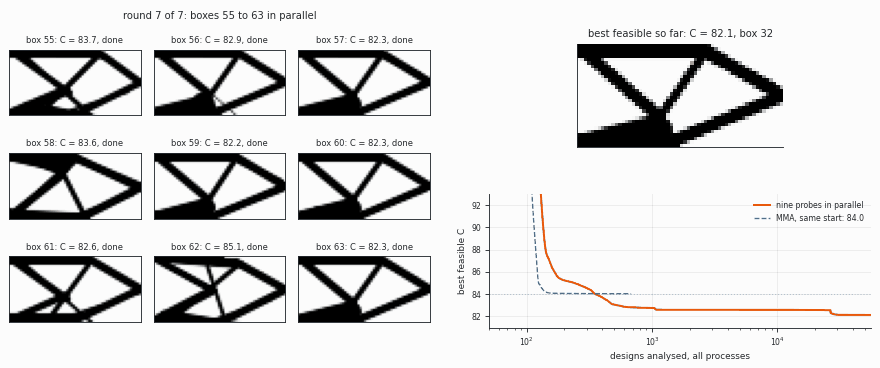
\includegraphics[width=\linewidth]{figures/cantilever_final.png}
  \caption{Box-subdivision method applied to the short cantilever problem. Left:
    the nine boxes of the last iteration of the master problem. Right: best
    feasible design ($C = 82.1$, box 32), and best feasible compliance as a
    function of the number of designs evaluated by all processes, compared with
    MMA from the reference initial design.}
  \label{fig:cantilever}
\end{figure}

From the reference initial design, MMA converges to the symmetric layout reported
by \citet{coniglio2020}, with $C = 84.0$ (Table~\ref{tab:cantilever},
Fig.~\ref{fig:cantilever}). The best compliance is $C = 83.0$ with the
multistart approach and $C = 82.1$ with the box-subdivision method, reached in
the 32nd box, the total numbers of evaluations being similar. With the same
budget, the classic tunneling method reaches $C = 82.8$, between the multistart
approach and the box-subdivision method, after $44\,072$ designs. The median
compliance over the $63$ runs is $95.6$ for the multistart approach and $83.8$
over the $63$ boxes for the method. The best layout is not symmetric, since the
lower diagonal bars meet the bottom chord at a single node instead of crossing
each other. The improvement with respect to the multistart
approach, about 1\%, is nevertheless modest, and is based on a single run of each
method. Moreover, the global optimum of this problem is unknown, and no
optimality certificate is provided by the method, so that the design with
$C = 82.1$ can only be regarded as the best design found among those evaluated,
without any claim of global optimality. The effect of the number of probes on
this problem is examined in Appendix~\ref{app:probes}.

%% ---------------------------------------------------------------------------
\section{Discussion}\label{sec:discussion}

\paragraph{Range of application.} The method is suited to landscapes with a
moderate number of well separated basins of attraction, for which a subdivision
can be found that separates the basins with fewer binary variables than the
number of sub-problems allowed by the budget. Under this condition, the optimum
is reached at an eighth to a third of the cost of the enumeration of the boxes
(Table~\ref{tab:enum}), the optimum of the Rastrigin function in five dimensions
is reached only by the method, from eleven starting points out of twenty
(Tables~\ref{tab:baselines} and~\ref{tab:tests}). Since the size of the master
problem depends on the number of binary variables and not on the number of
boxes, $10^5$ boxes can be handled in five dimensions. When no such subdivision
exists, the results are among the worst of the methods compared
(Table~\ref{tab:small}).

\paragraph{Safeguards against non-convexity.} The safeguard against
non-convexity determines the outcome of a run, and an inappropriate safeguard is
not detected by the method: a cut which overestimates the value function excludes
boxes without any error being reported (Section~\ref{sec:convexification}), and
a margin larger than the range of the objective function reduces the number of
starting points reaching the optimum (Table~\ref{tab:margin-ackley}). The
validity of the cuts, i.e. the absence of cuts which
overestimate the values observed at other boxes, and the sensitivities of the
sub-problem should therefore be verified when the method is applied to a new
problem.

\paragraph{Settings.} With the swept convexity, no parameter expressed in the
units of the objective has to be supplied. The swept configuration reached the
optimum at least as often as the calibrated one in
Tables~\ref{tab:variants}, \ref{tab:sweep} and~\ref{tab:sweep-density}, with the
exception of the Rastrigin function in five dimensions with ten subdivisions,
for which the difference is not significant. The trust-region radius is set to two changed
components, which is a suitable compromise for the problems studied but cannot
be regarded as a general rule. The subdivision density still has to be chosen.
The estimator based on basin counting provides a suitable density when its
estimate converges, and indicates when it does not, but its cost exceeds that of
a run.

\paragraph{Limitations.} The following limitations apply to the results
presented.
(i) The density, the number of probes, the trust-region radius and the headroom
factor of the sweep were selected on the problems on which they are evaluated.
(ii) Several results correspond to runs stopped by the budget; for the Ackley
function in five dimensions, doubling the budget changed the number of starting
points reaching the optimum from one to four out of twenty, and further increases
had no effect.
(iii) No convergence guarantee is obtained: with a large convexification
constant the optimality gap cannot close (Section~\ref{sec:convexification}),
and with the adaptive repair the runs can terminate on their own criterion away
from the optimum, as for the Rastrigin function in Table~\ref{tab:sweep-density}.
(iv) The analytic problems are only bound constrained, and the topology
optimization problem has a single volume constraint.
(v) The evaluation of the analytic functions takes a few microseconds, whereas
the method is intended for sub-problems whose solution takes minutes; neither
the cost of the master problem nor that of the surrogate model of efficient
global optimization is included in the budget. A comparison on an expensive
objective function is required to compare the method with Bayesian optimization.
(vi) Only the classic tunneling method was compared, with settings which were
not tuned; the variant applied with the geometry projection method
\citep{zhang2018tunneling}, and the filled function and deflation methods, were
not included in the comparison.

\paragraph{Future work.} Six directions of research follow from these results:
a least-squares repair with non-negative coefficients, which cannot increase a
cut at any box for one-hot variables;
a master problem defined over a growing set of boxes, in which the cuts are kept
when a box is refined, so that the hierarchies become a lazy branch and bound
procedure; the computation of a lower bound without the convexification term,
which would provide a meaningful optimality gap; a basin count accounting for
non-convex constraints such as stress constraints; the validation of the
swept convexity on an independent set of test problems; and a comparison with
the tunneling variant of \citet{zhang2018tunneling} and with deflation methods on
the same problems, including the topology optimization problem.

%% ---------------------------------------------------------------------------
\section{Conclusions}\label{sec:conclusion}

A box-subdivision outer approximation method has been presented, in which the
exploration of the design space is performed by a mixed-integer master problem
over one-hot box selections and the exploitation by a local gradient-based
optimizer within each box. The size of the master problem grows with the sum of
the subdivisions, and the cut slopes are obtained by post-optimal analysis
without additional evaluations. The method is effective when the subdivision
separates the basins of attraction and the number of binary variables remains
lower than the number of sub-problems allowed by the budget. Under these
conditions, the known global minimum of the Rastrigin function in five
dimensions, which none of the baselines reached, was found. For the short
cantilever problem of the generalized geometry projection, whose global optimum
is unknown, the best design found has a compliance of $82.1$, against $84.0$ for
the design obtained from the reference initial design, $83.0$ for a multistart
approach and $82.8$ for the classic tunneling method with the same budget. The
reliability of
the method depends on the safeguard against non-convexity and on a small
trust region measured in number of changed components; both lead to wrong
results without any warning when they are not set properly. The swept
convexity avoids the calibration of the only parameter expressed in the units of
the objective, and reached the optimum at least as often as the calibrated margin
in all but one of the configurations compared, for which the difference is not
significant. The admissible subdivision density
remains problem dependent, and its estimation by basin counting is affordable
only when the objective function is inexpensive.

%% ---------------------------------------------------------------------------
\backmatter

\bmhead{Acknowledgements}
\todo{Acknowledgements, if any.}

\section*{Declarations}

\bmhead{Funding}
\todo{Funding statement, or ``The author did not receive support from any
organization for the submitted work.''}

\bmhead{Conflict of interest}
The author declares no competing interests. \todo{confirm}

\bmhead{Replication of results}
The method, the benchmark problems, the baselines and the drivers of every
experiment are available in the open-source package \code{gemseo-box-subdivision},
version 0.3.0 \citep{boxsubdivision}, under the LGPL-3.0 licence. The analytic
experiments are reproduced with \code{tox -e benchmark}, and the data profiles
with \code{python -m benchmarks.data\_profiles}, whose output is distributed with
the documentation. The cantilever drivers are in \code{benchmarks/cantilever/}
and run in the environment of the GGP repository \citep{ggpcode}.
\todo{archive the release with a DOI (e.g.\ Zenodo) and cite it here.}

\bmhead{Use of generative AI}
\todo{The author must review and adapt this statement to what actually happened.}
The software, the numerical experiments and the documentation on which this
article is based were developed with the assistance of Claude (Anthropic), a
large language model used as a coding agent; the commits it produced are marked
as co-authored in the version history of the repository. A first draft of this
manuscript was generated with the same tool from the documentation of the
package. The author designed the study, directed and reviewed the
implementation and the experiments, checked the results and the text, and takes
full responsibility for the content of the article. In line with the policy of
the publisher, the language model is not listed as an author.

\bmhead{Author contributions}
\todo{CRediT statement, e.g.\ S.C.: conceptualization, methodology, software,
validation, writing.}

%% ---------------------------------------------------------------------------
\begin{appendices}

\section{Test problems}\label{app:problems}

\begin{table}[h]
  \centering
  \caption{Definitions, bounds and global minima of the test problems.}
  \label{tab:problems}
  \footnotesize\setlength{\tabcolsep}{4pt}
  \begin{tabular}{lll}
    \toprule
    problem & definition & bounds; minimum \\
    \midrule
    Rastrigin & $10n + \sum_i (x_i^2 - 10\cos 2\pi x_i)$ & $[-4.1, 5.9]^n$; $0$ at $0$ \\
    Ackley & $-20 e^{-0.2\sqrt{\frac1n\sum_i x_i^2}} - e^{\frac1n\sum_i\cos 2\pi x_i} + 20 + e$ & $[-28.7, 34.9]^n$; $0$ at $0$ \\
    Styblinski--Tang & $\frac12\sum_i (x_i^4 - 16x_i^2 + 5x_i)$ & $[-4.9, 5.1]^n$; $-39.166\,n$ at $x_i = -2.904$ \\
    Griewank & $1 + \frac{1}{4000}\sum_i x_i^2 - \prod_i \cos(x_i/\sqrt{i})$ & $[-58.1, 61.9]^n$; $0$ at $0$ \\
    partly multimodal & $\sum_{i\le 2}(10 + x_i^2 - 10\cos 2\pi x_i) + \sum_{i>2} x_i^2$ & $[-4.1, 5.9]^n$; $0$ at $0$ \\
    \bottomrule
  \end{tabular}
\end{table}

The gradients of all functions are computed analytically.

\section{Tuning of the master}\label{app:tuning}

Unless stated otherwise, the results of this appendix were obtained with the
adaptive repair and ten subdivisions per variable, from the twenty starting
points of Section~\ref{sec:baselines}, with a budget of $1000$ evaluations in two
dimensions and $2500$ evaluations in five dimensions.

\begin{table}[h]
  \centering
  \caption{Adaptive repair on Rastrigin, $n=2$: starting points reaching the
    optimum (median cost, when at least fifteen) against the number of parallel probes and the margin
    $\delta$.}
  \label{tab:margin}
  \small
  \begin{tabular}{lccccc}
    \toprule
    probes & $\delta = 1$ & 10 & 30 & 100 & 300 \\
    \midrule
    1 & 0/20 & 0/20  & 5/20        & 11/20        & 12/20 \\
    4 & 2/20 & 10/20 & 19/20 (360) & 19/20 (541)  & 20/20 (550) \\
    8 & 4/20 & 6/20  & 20/20 (905) & 20/20 (1000) & 19/20 (1000) \\
    \bottomrule
  \end{tabular}
\end{table}

\begin{table}[h]
  \centering
  \caption{Effect of the margin $\delta$ on Ackley, $n = 5$, $m = 10$ (range of
    the objective $14.5$): median distance, median cost and starting points
    reaching the optimum.}
  \label{tab:margin-ackley}
  \small
  \begin{tabular}{rrrrr}
    \toprule
    $\delta$ & fraction of the range & distance & cost & reached \\
    \midrule
    100 & 690\% & 6.302  & 2500 & 1/20 \\
    30  & 207\% & 4.945  & 2420 & 5/20 \\
    10  & 69\%  & 4.945  & 1814 & 5/20 \\
    3   & 21\%  & 7.076  & 1378 & 6/20 \\
    1   & 7\%   & 13.323 & 960  & 0/20 \\
    \bottomrule
  \end{tabular}
\end{table}

\begin{table}[h]
  \centering
  \caption{Convexification constant $\kappa$ on Rastrigin, one probe, adaptive
    repair disabled: median distance $\cdot$ starting points reaching the
    optimum.}
  \label{tab:constant}
  \small
  \begin{tabular}{lccccc}
    \toprule
    & $\kappa = 10$ & 30 & 50 & 100 & 200 \\
    \midrule
    $n=2$ & 11.44 $\cdot$ 0/20 & 0.00 $\cdot$ 18/20 & 0.00 $\cdot$ 14/20 & 0.00 $\cdot$ 15/20 & 0.00 $\cdot$ 12/20 \\
    $n=5$ & 34.61 $\cdot$ 0/20 & 19.19 $\cdot$ 1/20 & 1.99 $\cdot$ 5/20  & 1.99 $\cdot$ 2/20  & 2.99 $\cdot$ 2/20 \\
    \bottomrule
  \end{tabular}
\end{table}

\begin{table}[h]
  \centering
  \caption{Trust-region metrics, $n = 2$: median distance $\cdot$ median cost
    $\cdot$ starting points reaching the optimum. \emph{unit}: Hamming distance; \emph{none}: no trust
    region; \emph{proximity}: $|v^\top\alpha - v^\top\bar\alpha| \le \Delta$.}
  \label{tab:metric}
  \small
  \begin{tabular}{llll}
    \toprule
    metric, radius & Rastrigin & Ackley & Griewank \\
    \midrule
    unit, 2       & 0.000 $\cdot$ 541 $\cdot$ 19/20  & 0.000 $\cdot$ 528 $\cdot$ 17/20 & 0.007 $\cdot$ 743 $\cdot$ 0/20 \\
    unit, 1       & 0.000 $\cdot$ 458 $\cdot$ 20/20  & 0.000 $\cdot$ 454 $\cdot$ 20/20 & 0.007 $\cdot$ 530 $\cdot$ 0/20 \\
    none          & 0.000 $\cdot$ 845 $\cdot$ 20/20  & 0.000 $\cdot$ 591 $\cdot$ 15/20 & 0.007 $\cdot$ 1000 $\cdot$ 0/20 \\
    proximity, 3  & 0.000 $\cdot$ 1000 $\cdot$ 20/20 & 0.000 $\cdot$ 644 $\cdot$ 20/20 & 0.007 $\cdot$ 1000 $\cdot$ 0/20 \\
    \bottomrule
  \end{tabular}
\end{table}

\begin{table}[h]
  \centering
  \caption{Trust-region radius, $n = 5$: median distance $\cdot$ median cost
    $\cdot$ starting points reaching the optimum (Ackley and Griewank: median
    distance only, many runs being stopped by the budget).}
  \label{tab:radius}
  \small
  \begin{tabular}{rllll}
    \toprule
    radius & Rastrigin & Ackley & Styblinski--Tang & Griewank \\
    \midrule
    1 & 0.995 $\cdot$ 1232 $\cdot$ 7/20  & 6.01 & 0.000 $\cdot$ 395 $\cdot$ 16/20 & 0.027 \\
    2 & 0.000 $\cdot$ 1757 $\cdot$ 15/20 & 6.30 & 0.000 $\cdot$ 582 $\cdot$ 15/20 & 0.052 \\
    3 & 0.000 $\cdot$ 2049 $\cdot$ 15/20 & 7.08 & 0.000 $\cdot$ 773 $\cdot$ 20/20 & 0.036 \\
    5 & 0.000 $\cdot$ 2500 $\cdot$ 15/20 & 9.06 & 0.000 $\cdot$ 860 $\cdot$ 20/20 & 0.067 \\
    \bottomrule
  \end{tabular}
\end{table}

For the Rastrigin function, the results obtained with the adaptive repair no
longer improve above a threshold value of the margin, which increases with the
number of probes (Table~\ref{tab:margin}). For the Ackley function, whose range
is smaller than the calibrated margin, the optimum is reached most often for
intermediate values of the margin (Table~\ref{tab:margin-ackley}). The
convexification constant has a useful range bounded on both sides, and in five
dimensions none of the values tested reaches the optimum from more than five
starting points out of twenty (Table~\ref{tab:constant}). The Hamming distance
with a radius of one reaches the optimum of the Rastrigin and Ackley functions
from all starting points at the lowest cost among the metrics of
Table~\ref{tab:metric}, and the ordinal distance reaches it as often but at a
higher cost. In five dimensions, a radius of one reaches the optimum of the
Rastrigin function less often than the larger radii, and a radius of two that of
the Styblinski--Tang function less often than radii of three and five
(Table~\ref{tab:radius}). With ten subdivisions in five dimensions, the optimum
of the Rastrigin function is reached from at most five starting points with the
constant, against fifteen with the adaptive repair, which is therefore used by
default.

\section{Extensions}\label{app:extensions}

The results of this appendix were obtained in five dimensions with a budget of
$2500$ evaluations and the calibrated margin.

\begin{table}[h]
  \centering
  \caption{Partial subdivision of the partly multimodal function, twenty
    starting points: median distance, median cost and starting points reaching
    the optimum.}
  \label{tab:partial}
  \small
  \begin{tabular}{lrrrrr}
    \toprule
    subdivision & boxes & binaries & distance & cost & reached \\
    \midrule
    all 5 variables, $m=2$ & 32  & 10 & 1.99 & 506 & 0/20 \\
    3 variables, $m=4$     & 64  & 12 & 0.00 & 758 & 17/20 \\
    2 variables, $m=10$    & 100 & 20 & 0.00 & 990 & 20/20 \\
    2 variables, $m=5$     & 25  & 10 & 1.99 & 631 & 0/20 \\
    1 variable, $m=10$     & 10  & 10 & 3.98 & 420 & 5/20 \\
    \bottomrule
  \end{tabular}
\end{table}

\begin{table}[h]
  \centering
  \caption{Flat and multi-resolution encodings, twenty starting points: median
    distance (starting points reaching the optimum, when non-zero). $\dagger$
    median run stopped by the budget.}
  \label{tab:multires}
  \small
  \begin{tabular}{lrrlll}
    \toprule
    encoding & binaries & resolution & Rastrigin & Ackley & Styblinski--Tang \\
    \midrule
    flat, $m=10$          & 50 & 10 & 0.00 (15/20)  & 6.30$\dagger$ (1/20) & 0.00 (15/20) \\
    flat, $m=16$          & 80 & 16 & 1.99 (1/20)   & 5.53$\dagger$ (3/20) & 0.13 (10/20) \\
    $m=2$, $L=4$          & 40 & 16 & 3.06$\dagger$ & 13.15$\dagger$       & 9.32 (1/20) \\
    $m=2$, $L=5$          & 50 & 32 & 5.61          & 15.24$\dagger$       & 19.15 \\
    $m=4$, $L=2$          & 40 & 16 & 2.99 (2/20)   & 7.40                 & 3.81 (2/20) \\
    $m=4$, $L=3$          & 60 & 64 & 3.14 (1/20)   & 6.16$\dagger$        & 6.08 \\
    \bottomrule
  \end{tabular}
\end{table}

\begin{table}[h]
  \centering
  \caption{Hierarchies and flat subdivisions, twenty starting points: median
    distance, and, when non-zero, starting points reaching the optimum and median
    cost. $\dagger$ median run stopped by the budget; the frontier expands boxes
    until the budget is spent.}
  \label{tab:hierarchies}
  \small
  \begin{tabular}{llll}
    \toprule
    method & Rastrigin & Ackley & Styblinski--Tang \\
    \midrule
    flat, $m=2$               & 4.98                & 14.43                   & 0.00, 16/20, 481 \\
    flat, $m=10$              & 0.00, 15/20, 1757   & 6.30, 1/20, 2500$\dagger$ & 0.00, 15/20, 582 \\
    two levels, by value      & 4.98                & 6.30                    & 0.00, 16/20, 867 \\
    two levels, by cuts       & 2.99                & 9.58$\dagger$           & 0.00, 16/20, 974 \\
    deep, 4 levels of 2       & 4.98                & 0.00, 12/20, 2136       & 0.00, 16/20, 1490 \\
    frontier, best first      & 6.70$\dagger$       & 9.71$\dagger$           & 0.00, 20/20, 2500$\dagger$ \\
    \bottomrule
  \end{tabular}
\end{table}

\begin{table}[h]
  \centering
  \caption{Effect of the budget on Ackley, twenty starting points: median distance
    $\cdot$ median cost $\cdot$ starting points reaching the optimum.}
  \label{tab:budget}
  \small
  \begin{tabular}{rll}
    \toprule
    budget & flat, $m=10$ & deep, 4 levels of 2 \\
    \midrule
    2500     & 6.30 $\cdot$ 2500 $\cdot$ 1/20 (14 runs truncated) & 0.00 $\cdot$ 2136 $\cdot$ 12/20 \\
    5000     & 4.95 $\cdot$ 2620 $\cdot$ 4/20                     & 0.00 $\cdot$ 2575 $\cdot$ 12/20 \\
    10\,000  & 4.95 $\cdot$ 2620 $\cdot$ 4/20                     & 0.00 $\cdot$ 2575 $\cdot$ 12/20 \\
    \bottomrule
  \end{tabular}
\end{table}

\section{Number of probes for the cantilever problem}\label{app:probes}

The short cantilever problem of Section~\ref{sec:cantilever} was also solved with
nine and sixteen probes on the NumPy port of the reference code used for the
classic tunneling method, the other settings being unchanged and the probes
being solved over four processes. Since the iteration limit of the master
problem bounds its iterations and not the number of boxes, the two runs are
compared at the same numbers of designs evaluated: $31\,070$ and $55\,995$, the
numbers at which the run of Table~\ref{tab:cantilever} found its best design
and stopped (Table~\ref{tab:probes}).

\begin{table}[h]
  \centering
  \caption{Short cantilever problem on the NumPy port, one run for each number
    of probes: best feasible compliance and number of designs evaluated until
    the best design is found, for two numbers of designs evaluated.}
  \label{tab:probes}
  \small
  \begin{tabular}{lrrrr}
    \toprule
    & \multicolumn{2}{c}{$31\,070$ designs} & \multicolumn{2}{c}{$55\,995$ designs} \\
    \cmidrule(lr){2-3}\cmidrule(lr){4-5}
    probes & $C$ & to the best & $C$ & to the best \\
    \midrule
    9  & 82.58 & 24\,406 & 82.30 & 49\,032 \\
    16 & 82.58 & 18\,641 & 82.48 & 53\,299 \\
    \bottomrule
  \end{tabular}
\end{table}

After $31\,070$ designs, the same compliance is obtained with both numbers of
probes, sixteen probes reaching it after fewer designs. After $55\,995$ designs,
$C = 82.30$ is obtained with nine probes and $C = 82.48$ with sixteen. These
differences, based on one run for each number of probes, cannot be distinguished
from the variability between runs, and no advantage of sixteen probes is
observed on this problem. With nine probes, the compliance obtained on the port,
$C = 82.30$, differs from that of the reference implementation,
$C = 82.1$, so that the results of the two implementations are not compared with
each other.

\end{appendices}

\bibliography{references}

\end{document}
